\documentclass[9pt,twocolumn,twoside,lineno]{gsajnl}
\articletype{inv} % article type

\usepackage{amsmath,amssymb,amsthm}

\newcommand{\R}{\mathbb{R}}
\renewcommand{\P}{\mathbb{P}}
\newcommand{\E}{\mathbb{E}}
\newcommand{\var}{\mathop{\mbox{Var}}}
\newcommand{\cov}{\mathop{\mbox{cov}}}
\newcommand{\bone}{\mathbf{1}}
\newcommand{\st}{\,\colon\,}

% These macros are borrowed from TAOCPMAC.tex
\newcommand{\slug}{\hbox{\kern1.5pt\vrule width2.5pt height6pt depth1.5pt\kern1.5pt}}
\def\xskip{\hskip 7pt plus 3pt minus 4pt}
\newdimen\algindent
\newif\ifitempar \itempartrue % normally true unless briefly set false
\def\algindentset#1{\setbox0\hbox{{\bf #1.\kern.25em}}\algindent=\wd0\relax}
\def\algbegin #1 #2{\algindentset{#21}\alg #1 #2} % when steps all have 1 digit
\def\aalgbegin #1 #2{\algindentset{#211}\alg #1 #2} % when 10 or more steps
\def\alg#1(#2). {\medbreak % Usage: \algbegin Algorithm A (algname). This...
  \noindent{\bf#1}({\it#2\/}).\xskip\ignorespaces}
\def\kalgstep#1.{\ifitempar\smallskip\noindent\else\itempartrue
   \hskip-\parindent\fi
   \hbox to\algindent{\bf\hfil #1.\kern.25em}%
   \hangindent=\algindent\hangafter=1\ignorespaces}

\newcommand{\algstep}[3]{\kalgstep #1 [#2] #3 }
\newenvironment{taocpalg}[3]{%
\vspace{1em}%
\algbegin Algorithm #1. ({#2}). #3 }
{\vspace{1em}}

\newcommand{\algorithmref}[1]{#1}

\newtheorem{definition}{Definition}
\newtheorem{lemma}{Lemma}
\newtheorem{cor}{Corollary}
\newtheorem{theorem}{Theorem}
\newtheorem{example}{Example}

\newcommand{\tskit}{{\texttt{tskit}}}
\newcommand{\branch}{\mbox{Branch}} % branch stat
\newcommand{\branchp}{\mbox{Branch}_+} % polarised
\newcommand{\site}{\mbox{Site}} % site stat
\newcommand{\sitep}{\mbox{Site}_+} % polarised
\newcommand{\node}{\mbox{Node}} % node stat
\newcommand{\nodep}{\mbox{Node}_+} % polarised
\newcommand{\given}{\;\vert\;}

\newcommand{\treeseq}{\mathbb{T}} % tree sequence
\newcommand{\iw}{w} % sample (initial) weights
\newcommand{\tiw}{w_\text{total}} % total sample (initial) weights
\newcommand{\nw}{x} % subtree (node) weights
\newcommand{\aw}{{\bar x}} % allele weights

\newcommand{\Nt}{\mathcal{N}}  % node table
\newcommand{\Et}{\mathcal{E}}  % edge table
\newcommand{\prop}[1]{.\mbox{\texttt{#1}}} % property of a thing
% Not sure about this notation. Want to use i and o, but using normal
% math fonts would make things less clear, I think.
\newcommand{\indexin}[0]{\ensuremath{\mathbf{i}}}
\newcommand{\indexout}[0]{\ensuremath{\mathbf{o}}}
\newcommand{\plr}[1]{{\color{blue}\textbf{plr:} \it #1}}
\newcommand{\jk}[1]{{\color{red}\textbf{jk:} \it #1}}
\newcommand{\krt}[1]{{\color{green}\textbf{krt:} \it #1}}


\title{
    Efficiently summarizing relationships in large samples:
    a general duality between statistics of genealogies and genomes}

\author[$\ast$,1]{Peter Ralph}
\author[$\dagger$]{Kevin Thornton}
\author[$\ddagger$]{Jerome Kelleher}

\affil[$\ast$]{Institute of Evolution and Ecology, Departments of Mathematics and Biology, University of Oregon, Eugene, Oregon}
\affil[$\dagger$]{Department of Ecology and Evolutionary Biology, University of California, Irvine, California}
\affil[$\ddagger$]{Big Data Institute, Li Ka Shing Centre for Health Information and Discovery, University of Oxford}

\keywords{genealogy, tree sequence, genotype statistics}

\runningtitle{Genealogies and genomes}
\runningauthor{Ralph \textit{et al.}}


%%%%%%%%%%
\begin{abstract}
As a genetic mutation is passed down across generations,
it distinguishes those genomes that have inherited it from those that have not,
providing a glimpse of the genealogical tree relating the genomes to each other at that site.
Statistical summaries of genetic variation therefore also describe the underlying genealogies.
We use this correspondence to define a general framework that
efficiently computes single-site population genetic statistics
using the succinct tree sequence encoding of genealogies and genome sequence.
The general approach accumulates ``sample weights''
within the genealogical tree at each position on the genome,
which are then combined using a ``summary function'';
different statistics result from different choices of weight and function.
Results can be reported in three ways:
by \emph{site}, which corresponds to statistics calculated as usual from genome sequence;
by \emph{branch}, which gives the expected value of the dual site statistic
under the infinite-sites model of mutation,
and by \emph{node}, which summarizes the contribution of each ancestor to these statistics.
We use the framework to implement many currently-defined statistics of genome sequence
(making the statistics' relationship to the underlying genealogical trees concrete and explicit),
as well as the corresponding ``branch'' statistics of tree shape.
We evaluate computational performance using simulated data, and
show that calculating statistics from tree sequences using this general
framework is several orders of magnitude more efficient than
optimized matrix-based methods in terms of both run time and memory requirements.
We also explore how well the duality between site and branch statistics holds
in practice on trees inferred from the 1000 Genomes Project dataset,
and discuss ways in which deviations may encode interesting biological signals.
\end{abstract}

\begin{document}

\maketitle
\thispagestyle{firststyle}
\marginmark
\firstpagefootnote

\correspondingauthoraffiliation{1}{Corresponding author: {plr@uoregon.edu}}
\vspace{-33pt}% Only used for adjusting extra space in the left column of the first page


%%%%%%%%%%%%%%%%%%%%%%%
\section*{Introduction}

It was once a major undertaking to collect data sufficient to estimate a single summary
of the genetic relationships between the individuals of a
sample~\citep[e.g.,][]{Kreitman1983-xr}.
Today's vast quantity of whole-genome sequence
makes it possible to confidently estimate many more properties of genealogical relationships
in local regions of genomes, both between
individuals~\citep[e.g.,][]{browning2010highresolution,aguillon2017deconstructing}
and within
populations~\citep[e.g.,][]{booker2018understanding,haenel2018metaanalysis,stankowski2019widespread}.
Computation is beginning to be a major problem:
projects such as UK Biobank~\citep{bycroft2018genome}
and gnomAD~\citep{karczewski2019variation} hold genetic data for
hundreds of thousands of samples at tens to hundreds of millions of variant sites.
Such large genotype matrices are extremely unwieldy and difficult to process,
and computational complexity is usually linear in the size of the matrix.
Tools such as \texttt{Hail} (\url{https://hail.is}) allow computations to be sharded
across many machines in parallel, thereby calculating statistics far more
quickly than is possible using single-computer methods such as
\texttt{plink}~\citep{purcell2007plink}. Computer time must still be
paid for, however, and running calculations concurrently on thousands of cores quickly
becomes expensive. Larger datasets still, consisting of millions of whole
genomes, are currently being collected and it is clear that processing
and storing these genotype matrices will be very costly.

Genotype matrices are massively redundant, however, and several specialized
compression methods have been proposed~\citep{
christley2008human,qiao2012handling,durbin2014efficient,sambo2014compression,layer2016efficient,
danek2018gtc,lin2019sparse}.
The fundamental reason for this redundancy is that samples share ancestry:
related individuals will tend to share the same state at a particular variant site.
Trees describe these ancestral
relationships~\citep{felsenstein2004inferring,semple2003phylogenetics},
and provide a natural and elegant way of encoding genetic data,
not only recording the history of a sample but also massively compressing
the genotype matrix~\citep{ane2005missing}. Until recently, however,
tree based approaches could not be used to encode data from sexually reproducing organisms, because
recombination results in many trees along the
genome~\citep{hudson1983properties,griffiths1991two,griffiths1996ancestral,rasmussen2014genome},
and there was no efficient way of representing this information.
The \emph{succinct tree sequence} (or \emph{tree sequence}, for brevity)
is a recently introduced data structure that
encodes these genealogical trees along a genome concisely.
It was introduced in the context of coalescent
simulation~\citep{kelleher2016efficient}, leading to scalability increases of
several orders of magnitude over existing methods. The methods were subsequently extended
and refined for forwards-time
simulations~\citep{kelleher2018efficient,haller2018tree}, with similarly large efficiency gains.
Recent work has shown that tree sequence algorithms can
also be used to massively increase the scalability of methods for inferring
genome-wide genealogies, and making it possible to infer trees for millions of
samples~\citep{kelleher2019inferring}.
The key to the remarkable efficiency of tree sequence
algorithms is the way that shared structure in adjacent trees along the genome is encoded.
As one looks across the genome, genealogies change at recombination breakpoints in ancestors.
However, nearby trees tend to share much of their structure,
and single genealogical relationships (e.g., individual $x$ inherits from individual $y$)
are often shared across relatively long distances,
which manifest as shared \emph{edges} across many adjacent trees in the tree sequence.
This redundancy can be exploited to store genome sequence and the
associated genealogical relationships very compactly, and formed the basis for
efficient algorithms to calculate several population genetics
statistics~\citep{kelleher2016efficient}.
This paper generalizes the approach of \citet{kelleher2016efficient} to a much broader class of statistics,
supporting arbitrary tree topologies and patterns of allelic variation,
including polyallelic sites and back mutations.
% Want to emphasise generality here: people might assume we're only dealing
% with the biallelic case.

% summary
In this paper, we study ``single-site'' genetic statistics,
i.e., statistics of aligned genome sequence that can be expressed as averages over values computed
separately for each site. We develop a theoretical and computational framework
that encompasses a large class of population genetic statistics, generalizing
many classical summaries of genetic variation. We define
and explore a duality between ``Site'' and ``Branch'' statistics, and
provide a detailed description (and analysis) of an efficient algorithm
to compute statistics in this general setting.
The methods we describe are implemented, tested, and validated in the \tskit{}
Python and C libraries, freely available at \url{https://github.com/tskit-dev/tskit}
under the terms of the MIT license.

The basic relationship between tree shape and summaries of genetic variation
that we will explain and utilize below is this:
if mutations are neutral, then the expected number that occur on a
given branch of a tree is proportional to the length of that branch.
This ``duality'' (we will use the term more precisely later) has been
used extensively in deriving properties of statistics in models of random mating
\citep[e.g.,][]{tajima1983evolutionary,tavare1984lineofdescent,fu1995statistical},
as has the fact that it applies regardless of the underlying demographic model
\citep[e.g.,][]{gillespie1979evolutionary,hudson1983properties,slatkin1991inbreeding,
mcvean2002genealogical,lohse2016efficient,ralph2019empirical}. We build on this central
insight to define a flexible and computationally efficient framework for
population genetic statistics on tree sequences.
Roughly speaking, to compute a statistic we will
propagate ``weights'' additively up each marginal tree,
summarize these weights on each branch with a ``summary function'',
and aggregate these summaries to produce statistics.
Different choices of weights and summary functions
will then produce both familiar and novel statistics
of both genotypes and genealogies.

%%%%%%%%%%%%%%%%%%%%%%%
\section*{Framework and statistics}

Population genetic data is most directly represented as a matrix of genotypes,
and so summaries of population genetic data usually begin with this data structure.
However, since the genetic variation represented in a genotype matrix
was generated by mutations inherited through genealogical trees,
it is often informative to think about these statistics in terms of these trees.
Most population genetic summary statistics can be thought of in terms of the \emph{allele frequencies},
i.e., what proportion of some subset of the sampled genotypes carry each allele.
The frequency of any particular allele
can easily be found from the location of the mutation(s) that produced it
on the marginal genealogical tree,
by counting the number of sampled genotypes below the mutation(s) in the tree.
If many mutations have occurred at distinct sites that share a single genealogical tree,
then these mutations start to give us an idea of the shape of that tree.
This relationship is depicted in \autoref{fig:allele_freqs},
which shows the relationship between the genealogical tree
and the frequencies of alleles at five different sites across a region of the genome
described by that single tree.
Our goal will be to generalize this sort of summary of the genotype matrix,
using the underlying genealogical trees.
Working with the trees serves two purposes.
First, the trees are closer to the demographic processes that we are really interested in,
and so allow us to reason more directly about population genetic signal and noise.
Second, trees are highly efficient data structures,
and allow us to compute with genetic data far more efficiently than with the genotype matrix itself.


\begin{figure}
    \begin{center}
        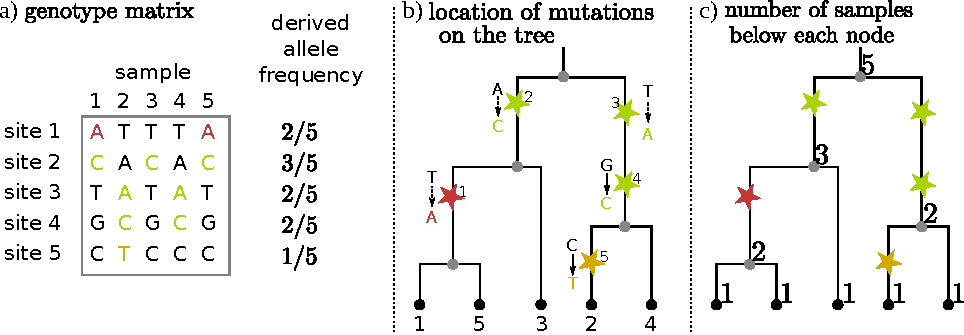
\includegraphics{figures/allele_frequency_diagram}
    \end{center}
    \caption{
        The relationship between allele frequencies and the underlying genealogical trees.
        \textbf{(a)} The genotype matrix, showing genotypes of five sequences (``samples'')
        at five separate sites,
        as well as the derived allele frequencies (derived alleles are shown in color,
        with separate colors for each genotype pattern:
        for example, all green mutations separate samples $s_1$, $s_3$ and $s_5$ from $s_2$ and $s_4$.
        \textbf{(b)} The genealogical tree describing how those five samples are related to each other
        over this segment of genome. The samples are leaves,
        and each mutation is represented as a star on the genealogy,
        with color matching the genotype matrix, and
        labeled with its index in the genotype matrix
        and the ancestral and derived states at that site.
        \textbf{(c)} Each node in the tree is labeled with the number of samples
        at or below that node, which we think of as a \emph{weight}.
        Note that this is \emph{additive}:
        the weight of each node is the sum of the weights of its child nodes.
        Since the frequency of a derived allele is the number of samples
        that have inherited that mutation, the allele frequency of each mutation
        is equal to the weight of the node directly below the mutation,
        divided by the total sample size.
        \label{fig:allele_freqs}
    }
\end{figure}

The operation of finding allele frequencies on a tree,
depicted in \autoref{fig:allele_freqs}(c)
is the basis of a familiar operation in population genetics:
summarizing the allele frequency spectrum.
Somewhat more generally, we could calculate how many of a certain set $A$ of samples
inherit from a particular branch in a tree
by (a) assigning each of these samples weight 1 (and other samples weight zero), then
(b) finding the total weight of all samples in the subtree inheriting from that branch.
This gives the number of samples that would inherit any mutation falling on this branch.
Suppose we want to calculate one of the linear functions of the frequency spectrum
discussed by \citet{fu1995statistical} and \citet{achaz2009frequency},
which can be described as follows.
Write $p_i(a)$ for the frequency of allele $a$ at a site $i$,
and $h(p)$ for the allele frequency spectrum
--- i.e., the number of alleles whose frequency is $p$ in our sample ---
and suppose that for some function $f()$, we want to compute $\sum_p h(p) f(p)$.
Since this is a simple sum over sites,
we can compute this by summing over the $L$ sites in the genome and all alleles
(including the ancestral allele),
\begin{align*}
    \sum_p h(p) f(p) = \sum_{i=1}^L \sum_a f(p_i(a)).
\end{align*}
For instance, mean genetic diversity across biallelic loci is computed using this formula
with $f(p) = p (1-p)$,
omitting the usual factor of two because the sum is over \emph{both} alleles at each site.
This is because genetic diversity is defined to be the probability that two randomly chosen sequences
differ at a randomly chosen site,
and the probability that two randomly chosen genomes differ at a site with allele frequency $p$
is $p (1-p) + (1-p) p$.
If we know where each mutation has occurred on the genealogical tree at each site in the genome,
we can easily compute statistics of this form
by finding allele frequencies, applying the function $f( )$ to each,
and summing up the results.

Our framework is somewhat more general than this, since we also define statistics that are
\emph{not} functions of the allele frequency spectrum.
The small but useful generalization we make is to allow the ``weights'' we propagate up the tree
to be numbers other than zero or one.
The general procedure is depicted in \autoref{fig:adding_weights}.
If weights \emph{are} all zero or one, then these weights will count numbers of samples
in each part of the tree;
but below we use other weights to compute the correlation between genotype and phenotype.

\begin{figure}
    \begin{center}
        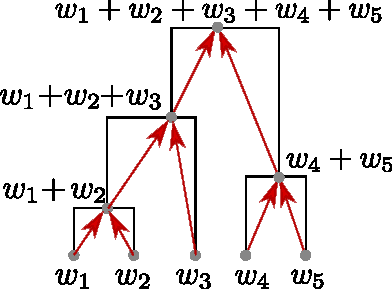
\includegraphics{figures/adding_weights}
    \end{center}
    \caption{
        \emph{Subtree weights} are assigned to each node by adding together the weights of any children,
        plus the weight of the node itself, if it is a sample.
        In this example, the samples are the five leaves, and have weights
        $\iw_1, \ldots, \iw_5$; the total weight -- also the subtree weight of the root --
        is $\tiw = \iw_1 + \cdots + \iw_5$.
        This can summarize the tree in many ways:
        for instance, if all weights were equal to one, then subtree weights would count the number of
        samples below that node.
        On the other hand, if $\iw_1 = 1$ but other weights were zero,
        then subtree weights would indicate whether a node was an ancestor of sample 1.
        If $\iw_k$ was the value of a phenotype of sample $k$,
        then the subtree weight of a node
        would equal the sum of all phenotypes inheriting from that node.
        \label{fig:adding_weights}
    }
\end{figure}

Before we formally describe the statistics, we need some notation and definitions.
A tree sequence describes how a set of $n$ sampled chromosomes
are related to each other along a (linear) genome of length $L$ \citep{kelleher2016efficient,kelleher2018efficient}.
Each haplotype, modern or ancestral, is associated with a \emph{node},
and the trees at each position along the genome have vertexes labeled by these nodes.
A tree sequence describes the relationships between a special set of nodes, the \emph{samples},
that appear in the trees at every point along the genome.
The other (non-sample) nodes may not appear in every tree,
as for instance if a portion of an ancestor's genome was not inherited by any of the samples.
From the tree sequence can be extracted a sequence of trees,
$\treeseq = (T_1, T_2, \ldots, T_{|\treeseq|})$
and a sequence of breakpoints $0 = a_0 < a_1 < \cdots < a_{|\treeseq|} = L$,
where $T_k$ describes the genealogical relationships of the samples
over the segment of genome between $a_{k-1}$ (inclusive) and $a_k$ (exclusive),
and $|\treeseq|$ is the number of trees.
We say that tree $T_k$ \emph{covers} the (half-open) segment $[a_{k-1}, a_k)$,
and call the length of this segment its \emph{span}, denoted $L_k = a_k - a_{k-1}$.
We refer to the branches in each tree using the most recent node,
so for instance a branch between an ancestor $v$ and descendant $u$
is associated with the node $u$.
Note that although the same parent-child relationship may exist across many adjacent trees
(this is called an ``edge''),
rearrangements of genealogical relationships due to recombination
can cause the precise set of samples that inherit from that edge to differ across trees.

\begin{definition}[Sample and subtree weights] \label{defn:weights}
    A list of \emph{sample weights} $\iw$ assigns a numeric value $\iw(v)$
    to every sample node.
    Given these weights,
    the \emph{subtree weight} $\nw_k(u)$ on tree $T_k$
    for a node $u$ is the sum of all sample weights
    of every sample node that is descended from $u$ in the tree (including $u$, if it is a sample):
    \begin{align*}
        \nw_k(u) = \sum_{v \,:\, v \le_{T_k} u} \iw(v) ,
    \end{align*}
    where $v \le_{T_k} u$ if $u$ is on the path from $v$ to root in the tree $T_k$.
    The \emph{total weight} is the sum of the weights over all samples:
    $\tiw = \sum_v \iw(v)$.
\end{definition}

If a given node $u$ is a sample and has no offspring (i.e., it is a leaf),
then its ``sample weight'' and ``subtree weight'' are the same: $\nw_k(u) = \iw(u)$.
However,
these differ for any samples that are internal nodes in a tree,
and so we use different notation to distinguish the two concepts.
Also note that $\tiw$ is the subtree weight of the root of any tree,
as long as the tree contains all the samples.

We allow vector-valued weights,
i.e., $\iw(v)$ may be a vector $(\iw_1(v), \ldots, \iw_m(v))$,
so that when summarizing we have access to more than one aspect of each subtree.
We will often be interested in statistics defined in terms of different subsets of our samples;
it is useful to have some additional notation to define these statistics.
Given a subset set $S$ of samples,
the \emph{indicator weights of $S$} are the sample weights $\bone_S$ with
$\bone_S(u) = 1$ if $u \in S$ and $\bone_S(u) = 0$ otherwise.

\begin{definition}[Summary function]
    For a set of $k$-dimensional weights with total weight $\tiw$,
    a summary function is any real-valued function $f(w_1, \ldots, w_k)$.
    We call the summary function \emph{strict} if $f(0) = f(\tiw) = 0$.
\end{definition}

The requirement that $f(0) = f(\tiw) = 0$ ensures
that statistics do not depend on portions of the tree either not ancestral to any of the samples
or ancestral to all of them.
This is desirable because genetic variation within the samples
cannot inform us about such parts of the tree.
However, as we will see below it is sometimes useful to use non-strict summary functions.
% Below, in section XXX, we describe how to efficiently
% maintain a list of the weights of the subtrees inherit from each node
% as we iterate through the tree sequence.


%%%%%%%%%%%%%%%%%%
% \subsection*{Tree sequences}

%%%%%%%%%%%%%%%%%%
\subsection*{Node statistics}

Perhaps the most natural way to summarize weights on the tree
is simply to examine the values at each node.
This would allow us, for instance, to
count the number of samples that inherit from each node in the tree.
Averaged across trees,
this tells us, for each node, what proportion of the sample's genomes were inherited from that node.
Motivated by this, we define the
\textbf{node statistic} for node $u$
associated with summary function $f()$ and sample weights $\iw$
to be the sum of $f()$ applied to the weight of the subtree inheriting from node $u$
and to the remaining weight of the rest of the tree,
averaged across the genome:
\begin{align}
    \node(f, \iw)_u
    =
    \frac{1}{L} \sum_{k=1}^{|\treeseq|} L_k \left( f(\nw_{T_k}(u)) + f(\tiw - \nw_{T_k}(u)) \right).
\end{align}
The weight $\nw_{T_k}(u)$ is the sum of the weights of all samples descending from node $u$
in the tree $T_k$,
and $\tiw - \nw_{T_k}(u)$ is the sum of all remaining weights.
This is an average over the genome because each tree is weighted by its span, $L_k$,
and the sum is divided by the total genome length,
which is the sum of all the spans: $L = L_1 + \cdots + L_{|\treeseq|}$.
If the node statistic is computed over only a ``window'' of the genome
then $L_k$ is replaced by the length of the portion of that window that the tree $T_k$ extends for,
and $L$ is replaced by the length of the window.

\paragraph{Polarization}
The node statistic defined above is appropriate for statistics of all alleles at given variable site.
For other statistics, one is only concerned with the derived state(s) at a site,
and we define a \emph{polarized} node statistic without the second term from our previous definition:

\begin{align}
    \text{(polarized)} \qquad
    \nodep(f, \iw)_u
    =
    \frac{1}{L} \sum_{k=1}^{|\treeseq|} L_k f(\nw_{T_k}(u)) .
\end{align}

\begin{example}[Ancestry proportions] \label{ex:ancestry_props}
    If $\iw = \bone_S$ are the indicator weights of the set $S$ of $n$ samples,
    then $\nw(u) / n$ is the proportion of the samples in $S$ that inherit from $u$.
    Therefore, if $f(x) = x / n$,
    then $\nodep(f, \iw)_u$ is the proportion of the genomes of $S$
    that are inherited from (ancestor) $u$.
\end{example}

Dividing this statistic by the total amount of the genome each node is ancestral to any samples,
we would obtain the ``genomic descent'' statistic defined by \citet{scheib2019anglian}.

Note that the summary function in this last example was not \emph{strict}, since $f(\tiw) \neq 0$.
Strictness is less important for node statistics than for the remaining classes of statistic,
because Node statistics only make sense in the context of the tree sequence.
However, Node statistics provide a useful bridge to the next type of statistic,
which are defined directly in terms of the genotypes.


%%%%%%%%%%%%%%%%%%
\subsection*{Site statistics}

Now we describe how to compute statistics from \emph{genomes} using this framework.
To do this, we assume that the genetic variation data is embedded in a tree sequence,
but the trees are used only for efficiency --- the results will not depend on
the trees in any way. The summaries we defined above for nodes
extend directly to genetic variants: just as a node weight contains information about
which samples inherit from the node and which do not,
so we can summarize patterns of genetic variation by summing up weights of all samples
that carry a given allele.
Therefore, we define \emph{allele weights} to be
the total weight of all sample nodes that have inherited that allele.

\begin{definition}[Allele weights]
    The \emph{allele weight} for allele $a$ at site $j$ is the sum of the weights
    of all sample nodes inheriting this allele:
    \begin{align*}
        \aw_j(a) = \sum_{v \st g_j(v) = a} \iw(v) ,
    \end{align*}
    where the sum is over all sample nodes $v$ for which
    $g_j(v)$, the allele carried by node $v$ at site $j$, is equal to $a$.
\end{definition}

If there has been only one mutation at the site,
then $\aw_j(a)$ is equal to the weight of the subtree inheriting from the mutation that produced $a$.
In the more general case of recurrent and back mutations, $\aw$ can
be computed from subtree weights in a straightforward way.
We then define the \textbf{site statistic} of site $j$ for a summary function $f()$
and sample weights $\iw$ to be the sum of $f()$
applied to the weight of every allele, $a$, found at this site:
\begin{align}
    \site(f, \iw)_j
    &=
    \sum_{a} f(\aw_j(a)).
\end{align}
Here, we think of a ``site'' as a single nucleotide position on the genome.
We often want to summarize statistics across regions of the genome (``windows'').
To do this, we overload notation somewhat and use a subscript $[i,j)$ to denote an average
over the corresponding portion of the genome:
\begin{align}
    \site(f, \iw)_{[i,j)}
    &=
    \frac{1}{j-i} \sum_{k=i}^{j-1} \site(f, \iw)_k
\end{align}
The requirement on strict summary functions that $f(0) = f(\tiw) = 0$
ensures that the sum is only affected by polymorphic sites,
although we normalize by total number of sites,
so that the values are comparable between different regions of the genome.


In the definition above we sum over all alleles at each site.
However, sometimes it is useful to distinguish the \emph{ancestral} allele
(i.e., the allele at the root of the tree) from the remaining derived alleles.
This allows statistics in principle to differentiate ancestral from derived alleles,
information which is available in practice (albeit noisily),
and one way to make use of this information is to sum over only derived alleles.
Analogously to the above,
we say a site statistic is \textbf{polarized} if we do this,
defining
\begin{align} \label{eqn:site_polarised}
    \text{(polarized)} \qquad
    \sitep(f, \iw)_j
    &=
    \sum_{a \in D_j} f(\aw_j(a)) ,
\end{align}
where $D_j$ denotes the set of all alleles at site $j$ except the allele at the root of the tree.
Note that this may not be quite what is expected,
for instance, if there has been a back mutation to the ancestral allele at some point in the tree,
or if there have been mutations to distinct alleles on different parts of the tree
such that the ancestral allele is no longer present.
However, since these situations depend on multiple mutations occurring at a single site,
they are relatively rare in practice.

Having defined a general framework, we may now give concrete examples
of how to compute common summary statistics.

\begin{example}[Nucleotide diversity] \label{ex:site_diversity}
    The nucleotide diversity of a group $S$ of $n$ samples
    is the average density of differences between pairs of samples,
    or equivalently, the average heterozygosity across positions.
    To calculate this statistic,
    % let $\iw_u = 1$ for $u \in S$ and $\iw_v = 0$ otherwise,
    let $\iw = \bone_S$,
    so that $\nw(u)$ gives the number of nodes in $S$ inheriting from $u$,
    and define
    \begin{align*}
        f(x) = \frac{x (n - x)}{n (n-1)} .
    \end{align*}
    Then $\site(f, \iw)_{[a,b)}$ is mean nucleotide diversity of $S$
    in the region of the genome between $a$ and $b$.
\end{example}

An alternative and possibly more familiar way to compute heterozygosity
would be to use a polarized Site statistic with summary function $f(x) = 2
x(n-x)/\left(n(n-1)\right)$.
However, this approach fails with more than two alleles per site.

\begin{example}[Nucleotide divergence] \label{ex:site_divergence}
    Now suppose we want to compute the mean pairwise density of nucleotide differences
    \emph{between} two nonoverlapping groups of samples, $S_1$ and $S_2$,
    with $n_1$ and $n_2$ samples, respectively.
    As before,
    let $\iw_j = \bone_{S_j}$,
    so that $\nw_{j}(u)$ gives the number of nodes in $S_j$ inheriting from $u$,
    and define
    \begin{align*}
        f(x_1, x_2) = \frac{x_1}{n_1} \left(1 - \frac{x_2}{n_2}\right) .
    \end{align*}
    Then $\site(f, \iw)_{[a,b)}$ is mean nucleotide divergence between the two groups
    in the region of the genome between $a$ and $b$.
\end{example}

The procedure of computing divergence at a single site is shown in \autoref{fig:divergence_diagram};
divergence over a region of the genome would sum these values across all polymorphic sites
and divide by the length of the region.

\begin{figure}
    \begin{center}
    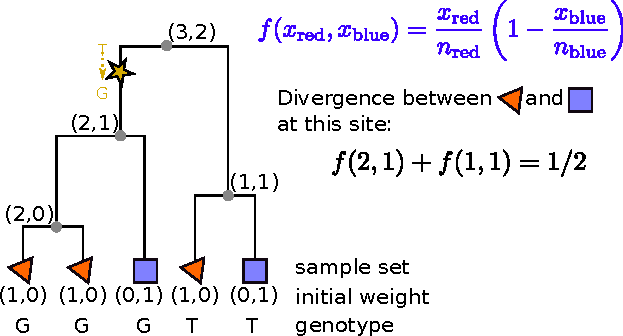
\includegraphics{figures/divergence_diagram_simple}
    \end{center}
    \caption{
        An example of computing sequence divergence
        between red samples (triangles) and blue samples (squares)
        at a single site with a T$\to$G mutation, using the tree.
        Each node is labeled with subtree weights $(x_\text{red},x_\text{blue})$,
        recording how many red samples ($x_\text{red}$)
        and how many blue samples ($x_\text{blue}$) lie in that subtree.
        The derived mutation is found in $x_\text{red}=2$ out of the $n_\text{red} = 3$ red samples
        and in $x_\text{blue}=1$ of the $n_\text{blue}=2$ blue samples, and so the probability that a randomly chosen red node carries the derived allele
        but a randomly chosen blue node does not
        is given by the summary function, $f(x_\text{red}, x_\text{blue}) = f(2, 1) = 2/6$.
        The complementary value, $f(1, 1) = 1/6$ is the probability that the mutation separates
        a randomly chosen red and blue pair, but with the blue node carrying the derived allele,
        so the total probability that a randomly chosen pair
        differs at this site is $f(2,1) + f(1,1) = 1/2$.
        \label{fig:divergence_diagram}
    }
\end{figure}

\begin{example}[Segregating sites] \label{ex:segregating_sites}
    Again, let $\iw = \bone_{S}$ for a group of $n$ samples,
    and now define
    \begin{align*}
        f(x) = \begin{cases}
            1 - \frac{x}{n} \qquad &\text{if } x > 0 \\
            0 \qquad &\text{otherwise} .
        \end{cases}
    \end{align*}
    In computing $\site(f, \iw)_{[a,b)}$, the argument $x$ to the function $f(x)$
    is the number of samples in $S$ that inherit each allele.
    A site with $k$ distinct alleles that segregate in $S$ with counts $x_1 + \cdots + x_k = n$
    contributes $f(x_1) + \cdots + f(x_k) = (1 - x_1/n) + \cdots + (1 - x_k/n) = k - 1$
    to the statistic.
    Therefore, $\site(f, \iw)_{[a,b)}$, is the minimum number of derived mutations per unit length,
    which is the density of segregating sites if all sites are biallelic.
    (The actual number of mutations per unit length will be greater if there have been back mutations.)
\end{example}

\paragraph{Polyallelic sites}
The summary function in Example~\ref{ex:segregating_sites} might be surprising:
the reason for its particular form is so that the statistic returns a sensible answer
even when sites may have more than two alleles.
There is not a consensus in the field
on how to use sites with more than two alleles, but the most common practice is
to reduce to biallelic data, by either discarding other sites
or by marking all non-ancestral alleles as (the same) ``derived'' allele.
In contrast, we choose to define statistics in a way that still makes formal sense for polyallelic sites,
so that for instance a site with ancestral allele $A$ and derived alleles $C$ and $T$
would have site statistic $f(\aw(A)) + f(\aw(C)) + f(\aw(T))$.
This is not the only choice, but is natural because it agrees with what is obtained by
looking at pairwise haplotype differences.
For instance, the definition of nucleotide divergence in Example \ref{ex:site_divergence}
gives the probability that a randomly chosen sample from each set differ,
a definition that makes sense even with polyallelic sites.


\begin{example}[Phenotypic correlations] \label{ex:site_correlations}
    Suppose that for each sample $u$ we have a numeric phenotype, denoted $z(u)$,
    and we want to compute the correlation between this phenotype
    and the genotype at each site.
    For convenience, suppose $z$ is normalized
    % so that $\sum_u z(u) = 0$ and $\sum_u z(u)^2/(n-1) = 1$.
    to have mean zero and variance 1.
    Then, if $g_j$ is a vector of binary genotypes (so $g_j(u) = 1$ if $u$ carries the derived allele),
    then the covariance of $z$ with $g_j$ is just $\sum_u z(u) g_j(u) = \sum_{u \st g_j(u) = 1} z(u)$,
    i.e., the sum of the phenotypes of all samples carrying the derived allele,
    divided by $(n - 1)$, where $n$ is the number of samples.
    Since the phenotypes sum to zero, this is also equal to
    $- \sum_{u \st g_j(u) = 0} z(u)$.
    If $p_j = \sum_u g_j(u)$ is the derived allele frequency at site $j$,
    then the variance of $g_j$ is $n p_j (1-p_j) / (n-1)$,
    and so the squared correlation can be calculated as a sum across the two alleles:
    \begin{align*}
        r_j^2 =
        \frac{\left( \sum_{u \st g_j(u) = 0} z(u)\right)^2}{2p(1-p)n(n-1)}
        + \frac{\left( \sum_{u \st g_j(u) = 1} z(u)\right)^2}{2p(1-p)n(n-1)}  .
    \end{align*}
    We can compute this as a site statistic by defining $\iw_{1}(u) = z(u)$, and $\iw_{2}(u) = 1/n$,
    and $f(x_1, x_2) = x_1^2 / (2 x_2 (1 - x_2) n (n-1))$:
    then $\site(\iw, f)_j = r_j^2$ is the squared correlation between $z$ and the allele at site $j$.
\end{example}

Appendix \ref{apx:regression} explains how to extend the previous example
to obtain the squared coefficient of genotype in the regression of phenotype
against genotype with additional covariates.

%% Check that math:
% n <- 10; z <- rnorm(10); z <- (z - mean(z))/sd(z); g <- rbinom(n, size=1, prob=1/2); p <- mean(g)
% c(cov(z,g), sum(z*g)/(n-1))
% c(cor(g,z), sum(g*z)/sqrt(n*(n-1)*p*(1-p)))
\begin{example}[Patterson's $f_4$] \label{ex:site_f4}
    Given four disjoint groups of samples, $S_1$, $S_2$, $S_3$, and $S_4$,
    Patterson's $f_4(S_1, S_2; S_3, S_4)$
    statistic~\citep{reich2009reconstructing,patterson2012ancient}
    for an allele with frequency $p_i$ in group $S_i$
    is $(p_1 - p_2)(p_3 - p_4)$. To rewrite this as a sum over alleles, note that
    $p_1 - p_2 = p_1 (1 - p_2) - (1 - p_1) p_2$,
    and so the statistic counts with positive value
    alleles that split $S_1$ and $S_3$ from $S_2$ and $S_4$,
    and negative value ones that split $S_1$ and $S_4$ from $S_2$ and $S_3$.
    Therefore, if as before we
    let $\iw_j = \bone_{S_j}$
    % let $\iw_{ju} = 1$ if $u \in S_j$
    (so that $\iw_{j}(u)$ tells us the number of samples in $S_j$ descended from $u$),
    and write $n_i$ for the number of samples in $S_i$, and
    \begin{align*}
        f(x_1, x_2, x_3, x_4)
        =
        \frac{x_1}{n_1}
        \left(1 - \frac{x_2}{n_2}\right)
        \frac{x_3}{n_3}
        \left(1 - \frac{x_4}{n_4}\right)
        -
        \left(1 - \frac{x_1}{n_1}\right)
        \frac{x_2}{n_2}
        \frac{x_3}{n_3}
        \left(1 - \frac{x_4}{n_4}\right),
    \end{align*}
    then $\site(\iw, f)_{[a,b)}$ is equal to Patterson's $f_4(S_1, S_2; S_3, S_4)$ statistic
    for the region of the genome between $a$ and $b$.
\end{example}

Again, we have taken care so that this definition
makes sense even with more than two alleles per site.
This definition of $f_4$ can be restated as follows:
averaged across a random choice of individuals from the four groups of samples,
let ``BABA'' be the proportion of sites at which samples 1 and 3 agree,
but differ from samples 2 and 4 (which may differ from each other as well);
and let ``ABBA'' be the proportion of sites at which 2 and 3 agree, but differ from 1 and 4;
then $f_4$ is BABA minus ABBA.
In this mnemnonic, B is standing in for a \emph{specific} allele, that must match;
but A is standing in for ``any allele that is not B''.
This is more general than previous definitions, but agrees with them for biallelic sites.


%%%%%%%%%%%%%%%%%%
\subsection*{Branch statistics}

Genetic variation is informative about many processes
precisely because it tells us about the underlying patterns of genealogical relatedness.
In other words, often the genomes are most useful in so far as they tell us about the trees.
In the case where we actually have the trees, or a good proxy for them,
it is natural to summarize them directly rather than working indirectly with the
genotypes~\citep{harris2019database}.
If we assume that no two mutations occur at the same genomic position ---
i.e., the \emph{infinite sites model} ---
then there is a natural correspondence between summaries of genotypes and summaries of tree shape.
If mutations occur at a constant rate in time and along the genome,
then the \emph{expected} number of mutations that occur somewhere along a branch of a tree
over some segment of genome
is equal to the mutation rate multiplied by the length of the segment and by the length of the branch.
In other words, the ``area'' of a branch in a tree,
defined as its span (right minus left endpoint) multiplied by its length (parent time minus child time)
and scaled by the mutation rate,
is equal to the expected number of mutations that will land on it.
If the mutation rate is constant,
then this gives us an isometry:
tree distances measured in branch lengths versus in numbers of mutations
are equal in expectation, up to a multiplicative factor of the mutation rate.

This makes it natural to define
a statistic of tree shape by summing these expected contributions across its branches.
We define the \textbf{branch statistic} of the $k^\text{th}$ tree $T_k$,
obtained from summary function $f()$ and sample weights $\iw$,
to be the sum of the length of each branch
multiplied by the summary function applied to its subtree weight
and the remaining weight not in the subtree:
\begin{align}\label{eqn:branch_stat_tree}
    \branch(f, \iw)_k
    &=
    \sum_{u \in T_k} \beta_{k}(u) \left( f(\nw_{k}(u)) + f(\tiw - \nw_{k}(u)) \right)  .
\end{align}
Here, $\beta_{k}(u)$ is the length of the branch between $u$ and its immediate ancestor in tree $T_k$,
$\tiw = \sum_u \iw(u)$ is the total weight,
and $\nw_{k}(u)$ is the total weight of the subtree of $T_k$ inheriting from $u$ (as defined above).
The term $\tiw - \nw_{k}(u)$ gives the total weight \emph{not} in the subtree of $T_k$ inheriting from $u$.
The value $f(\nw(u))$ is the summary value that would be added to a site statistic
if a single mutation occurred on the branch ancestral to $u$,
and $f(\tiw - \nw_{k}(u))$ is the value that would be added due to its complementary allele,
so $\branch(f, \iw)_k$ gives the expected contribution of the tree $T_k$ to $\site(f, \iw)$,
per unit of sequence length that the tree covers.
An example of this correspondence between site and branch statistics
is shown in Figure~\ref{fig:branch_site_diagram}. Here, we
see how the $f_4$ site statistic assigns a weight to each mutation
depending on its frequency in each of the four sample sets,
and how the corresponding branch statistic assigns the same weight to those branches.

\begin{figure}
    \centering
    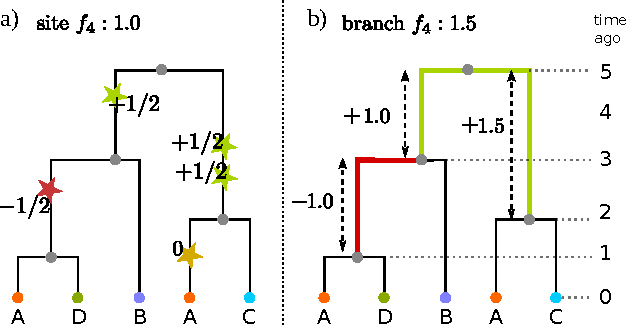
\includegraphics[width=\textwidth]{figures/branch_site_diagram}
    \caption{
    Computing the $f_4(A,B;C,D)$ statistic on a tree,
    for groups of genomes labeled $A$, $B$, $C$, and $D$
    (only group $A$ has more than one sample),
    on the same basic example as Figure \ref{fig:allele_freqs}.
    \textbf{(a)} The genotype matrix, for five sampled genomes at five sites.
    Also shown are the derived allele frequencies in each of the four groups,
    denoted by $p_A$, $p_B$, $p_C$, and $p_D$ respectively.
    \textbf{(b)} Each mutation is given weight equal to $(p_A - p_B)(p_C - p_D)$,
    shown as a label next to each mutation (depicted as a star),
    and the Site $f_4(A,B;C,D)$ statistic is the sum of these weights
    divided by $L$, the sequence length.
    Note that each of the mutations shown occurs at a distinct site, so there is no back mutation,
    and that all mutations on the same branch have the same weight.
    \textbf{(c)} Each branch is assigned weight equal to the weight that would be assigned
    to any mutation falling in it (colored lines, with colors matching the mutations of (b)),
    and then the branch $f_4$ statistic
    is the sum over these weights, multiplied by the length of the branch,
    and divided by $L$, the sequence length.
    Remaining branches do not contribute,
    because any mutation falling on these have either $p_A - p_B = 0$ or $p_C - p_D = 0$.
        \label{fig:branch_site_diagram}
    }
\end{figure}

Equation~\eqref{eqn:branch_stat_tree} defines a statistic for a single tree,
but in practice it is more useful to average branch statistics
over a region of the genome, as we did for Site statistics.
We do this by averaging the tree statistics over the region
with probabilities proportional to the trees' spans:
\begin{align}
    \branch(f, \iw)_{[i,j)}
    &=
    \frac{1}{j-i} \sum_{k=1}^{|\treeseq|} \ell_k(i,j) \branch(f, \iw)_{k} ,
\end{align}
where $\ell_k(i,j)$ is the length of the region in $[i,j)$ that the tree $T_k$ covers
(i.e., if $T_k$ covers the half-open interval $[a_{k-1},a_k)$,
then $\ell_k(i,j) = \max(0, \min(j,a_k) - \max(i,a_{k-1}))$).
The \emph{polarized} version of a Branch statistic
is defined analogously to the Node and Site versions:
\begin{align} \label{eqn:branch_polarised}
    \text{(polarized)} \qquad
    \branchp(f, \iw)_k
    &=
    \sum_{u \in T_k} \beta_{k}(u) f(\nw_{k}(u)) ,
\end{align}
and $\branchp(f, \iw)_{[i,j)}$ is defined using $\branchp(f, \iw)_k$ as before.

\begin{example}[Mean TMRCA] \label{ex:branch_diversity}
    If we take $\iw$ and $f$ exactly as in the ``Nucleotide diversity'' example above,
    then $f(u)$ gives the probability that the branch between $u$ and its ancestor in the tree
    lies on the path from one of two randomly chosen samples from $S$
    on the path up to their most recent common ancestor (MRCA).
    Therefore, $\branch(f, \iw)$
    gives the mean total distance in the tree between two samples from $S$,
    averaged across the sequence.
    This is twice the mean time back to the MRCA if the samples are all from the same time.
\end{example}

\begin{example}[Phenotypic correlation with pedigree] \label{ex:branch_correlation}
    If we take $\iw$ and $f$ as in the ``Phenotypic correlations'' example above,
    then $\branch(f, \iw)$ gives the \emph{expected} correlation between phenotype and any mutations
    appearing on the tree. This is a summary of how much local relatedness
    aligns with similarity in phenotype.
\end{example}

The previous example might be used to leverage local relatedness
to improve the resolution of association studies.
Similar strategies were explored by \citet{zollner2005coalescent} and \citet{minichiello2006mapping}.

\begin{example}[Patterson's $f_4$] \label{ex:branch_f4}
    Suppose that the four subsets each consist of only a single sample.
    The summary function $f(x_1, x_2, x_3, x_4)$ for the $f_4$ statistic
    then assigns weight 1 to any branch that separates $x_1$ and $x_3$ from $x_2$ and $x_4$,
    and weight -1 to any branch that separates $x_1$ and $x_4$ from $x_2$ and $x_3$.
    The statistic $\branch(f, \iw)$ therefore
    gives the difference in average lengths of these two types of branch,
    averaged across the genome.
\end{example}



%%%%%%%%%%%%%%%%%%
\section*{Duality of site and branch statistics}

Under a neutral, infinite-sites model of mutation with constant mutation rate across time,
the expected number of mutations per branch is proportional to its length.
This implies an isomorphism between ``Site'' and ``Branch'' statistics defined above,
which is discussed in more detail in \citet{ralph2019empirical}.
For instance, the site statistic of Example \ref{ex:site_diversity} (genetic diversity)
and the branch statistic of Example \ref{ex:branch_diversity} (mean TMRCA)
use the same summary function $f(x) = x(n-x)/\left(n(n-1)\right)$.
These are closely related because under an infinite-sites model of mutation,
two sequences differ at a site only if there has been a mutation somewhere on the branches going back
to their most recent common ancestor.
Therefore, if mutations occur with constant rate
the expected value of genetic diversity
% averaging over mutational noise given the tree sequence,
is equal to the mutation rate multiplied by the average path distance between
the two samples in the trees.

This relationship is true more generally.
In fact, for any region of the genome between $i$ and $j$,
% with $\treeseq_{[i,j)}$ the trees spanning that interval,
\begin{align}
    \branch(f, \iw)_{[i,j)}
    =
    \frac{1}{\mu}
    \E\left[ \site(f, \iw)_{[i,j)} \given \treeseq_{[i,j)} \right].
\end{align}
Here, $\treeseq_{[i,j)}$ denotes the tree sequence on the interval $[i,j)$,
and so the expectation keeps the genealogies fixed
and averages over infinite-sites mutations
with rate $\mu$ per unit time and per unit of sequence length.
Note that the expected product of two site statistics,
$\E[\site(f, \iw) \site(g, \iw') \given \treeseq]$
is not equal to the product of the two branch statistics, $\mu^2 \branch(f, \iw) \branch(g, \iw')$,
because they are not independent.
However, it is always possible to define a branch statistic that
gives the expected value of the product, as described in \citet{ralph2019empirical}.

A Site statistic can therefore be thought of as an estimator of its corresponding Branch statistic,
which is itself a summary of local tree shapes.
Because we have normalized these statistics by the length of the genome under consideration,
both sides of this equation are in units of \emph{time}:
Branch statistics give mean weighted branch lengths;
Site statistics give mean densities of mutations per unit of sequence length,
which divided by the mutation rate $\mu$ is converted to time.
Let's unpack the assumptions here: what exactly is the mutational model?
First, we are taking the mutation rate to be $\mu$, i.e.,
the expected number of mutations that occur on a region of the genome of length $\ell$
over $t$ units of time is equal to $\mu \ell t$.
Second, we are assuming that the probability of per-site mutation is low enough
that no two mutations occur at the same site
--- the fact that they do, occasionally, means that this is an approximation.
Third, we are assuming that mutation rates are constant through time and across the genome.
Of course, the statement remains true if we can measure distance along the genome and time
in a way that mutation rates are constant, but how these vary is generally unknown.

In this view,
site statistics are noisy approximations to the corresponding branch statistic
--- but, how noisy?
How big is the contribution of mutation to the overall sampling variance of a statistic?
The law of total variance partitions the variance of a site statistic
into the contributions of noise from demography and mutation:
\begin{align*}
    \var[\site(f, \iw)_{[i,j)}]
    &=
        \var\left[ \E\left[\site(f, \iw)_{[i,j)} \given \treeseq_{[i,j)}\right] \right]
            +
        \E\left[ \var\left[\site(f, \iw)_{[i,j)} \given \treeseq_{[i,j)}\right] \right]
        \\
    &=
        \mu^2 \var\left[ \branch(f, \iw)_{[i,j)} \right]
            +
        \frac{\mu}{j-i} \E\left[ \branch(f^2, \iw)_{[i,j)} \right] .
\end{align*}
The first term is the variance of the expected Site statistic given the trees,
which by duality is the variance of the Branch statistic,
i.e., the contribution of demographic noise, including genetic drift.
The second term, the expected variance of the statistic given the trees,
is the contribution to variance of mutation,
and can itself be written as a Branch statistic,
using the same weights and the summary function $f(x)^2$
\citep[Lemma 2 in][]{ralph2019empirical}.
The reason for this is straightforward ---
the Site statistic is a sum across branches of the number of mutations on the branch
multiplied by a summary, $f(x)$.
Given the trees, these numbers of mutations are independent and Poisson,
and the variance of the product of the constant $f(x)$
and a Poisson random variable with mean $m$ is $m f(x)^2$.
The sum is divided by the length of the region, $j-i$,
and so the variance is divided by $(j-i)^2$,
but one factor of $(j-i)$ is absorbed by the definition of the branch statistic.


We examined the contributions of mutation and demography to noise
in two simulations where population genetic (Site) statistics
are important in making inferences:
detecting recent selective sweeps,
and detecting introgression.
\autoref{fig:sweep_duality} shows windowed
diversity along the chromosome following a few selective sweeps.
The top two plots compare Branch diversity --- i.e., as computed only with tree shape ---
to Site diversity computed from sequences generated by 20 independent assignments of mutations to the same tree sequence,
with mutation rates $10^{-9}$ and $10^{-8}$, respectively.
We see that as the mutation rate increases, the signal of decrease in diversity around swept loci becomes more clear,
and Site diversity approaches Branch diversity.
These were computed using the entire population of 1,000 individuals;
how does sampling variance contribute?
Not much, it turns out --- the bottom plot shows both Site and Branch diversity
computed from 20 nonoverlapping groups of 100 samples.
Neither Site or Branch diversity vary much between these samples,
implying that the subsample gives us a good estimate of the whole-population values of each.
However, as we see in the top figure,
whole-population Site diversity is itself only a quite noisy estimator of Branch diversity.
(Note, however, that statistics other than diversity may vary much more between subsamples.)
The same things are shown in Supplementary Figure \ref{sfig:sweep_duality_10K}
for a simulation with 10,000 individuals, which shows similar patterns.
Only the last of these plots is possible to directly observe in real data:
in the top two plots,
the spread of independent replicates of mutational noise (black lines)
about their expectation based on the tree sequence (red line)
is unobservable, although estimable.


\begin{figure}
\centering
    \includegraphics[width=0.8\textwidth]{{figures/swept.1000.999.1e-09.diversity}.pdf}
    \caption{
        Mean genetic diversity and time to most recent common ancestor
        in 500Kb windows along a 50Mb genome (0.5 Morgans) following several selective sweeps.
        In each case, ``site'' is mean genetic diversity (Tajima's $\pi$) divided by mutation rate,
        and ``branch'' is the corresponding Branch statistic.
        The tree sequence was produced by simulating mutations under positive selection with mutation rate $10^{-12}$
        in a population of size 1000 for 400 generations using SLiM,
        followed by recapitation with $N_e=1000$~\citep{haller2018tree}.
        The selected alleles at the marked sites have selection coefficients between 0.08 and 0.25,
        and are at frequencies 96.8\%, 100\%, 100\%, and 82.6\% in the final generation, respectively.
        All curves use the same tree sequence, including selected mutations,
        but with additional neutral mutations added.
        \textbf{(top)}
        Diversity within the entire population,
        computed as a Site statistic from 20 independent assignments of mutations to the same tree sequence with mutation rate $\mu = 10^{-9}$.
        \textbf{(middle)}
        As in the top panel, but with mutation rate $\mu=10^{-8}$,
        showing that as mutation rate increases, the Site statistic (divided by $\mu$)
        converges to the Branch statistic.
        \textbf{(bottom)}
        Site and Branch diversity within 20 disjoint samples of size 100 each
        from a \emph{single} assignment of mutations to the tree sequence
        with mutation rate $\mu = 10^{-9}$.
        \label{fig:sweep_duality}
    }
\end{figure}


As another example, we simulated an ``admixture'' scenario:
a first population of size $N=1000$ splits into two of equal size,
then after $N$ generations, the second population splits,
after another $N$ generations, the third population splits again,
and for the final $N$ generations populations 2 and 3
have per-capita migration rates of $4/N$ to each other.
We expect a negative $f_4(1,2;3,4)$ in this situation,
which we indeed find
(the genome-wide mean Branch $f_4$ is around -700 generations,
as is the Site $f_4$ divided by mutation rate;
see Supplemental Figure~\ref{fig:introf4} for a plot along the genome).
Using various sample sizes, mutation rates, and window sizes, we then
calculated this $f_4$ statistic in windows along a 100Mb genome,
and show the standard deviation of both Site and Branch statistics across windows
in Figure~\ref{fig:introf4sd}.
Since the genome is uniform (no selection or variation in recombination or mutation),
this standard deviation is a measure of noisiness.
As expected, Site statistics are noisier than Branch statistics,
by a factor that depends mostly on the ratio of mutation to recombination rates.
The results suggest that Branch statistics would provide substantially better resolution
at small scales along the genome, especially if mutation rate is lower than recombination rate.
However, in practice imperfect estimation of the tree sequence
would introduce additional noise,
so it remains to be seen if the improvement could be made in practice.

\begin{figure}
    \includegraphics{{figures/intro/introgressed.1000.23.10000.1e-09.f4sd}.pdf}
    \caption{
        Standard deviation of Site (black) and Branch (red) $f_4(1,2;3,4)$
        in windows along a 100Mb genome, as a function of
        \textbf{(left)} mutation rate,
        \textbf{(middle)} sample size, and
        \textbf{(right)} window width.
        The recombination rate was $10^{-8}$,
        and unless otherwise stated, the mutation rate was $10^{-9}$,
        the window width was 10Kb,
        and the entire population (1000 diploids in each of four populations) was used.
        \label{fig:introf4sd}
    }
\end{figure}


%%%%%%%%%%%%%%%%%%%%%%%
\section*{Data and code availability}

All methods described here are implemented in Python and C in the package \tskit{},
available from \url{https://github.com/tskit-dev/tskit}
under the terms of the MIT license.
All code used to produce the figures in this paper
is available from \url{https://github.com/petrelharp/treestats_ms}.

%%%%%%%%%%%%%%%%%%
\section*{Application to 1000 Genomes tree sequences}

We do not know the true genealogies underlying real data,
but recent methods are available to estimate them at
scale~\citep{kelleher2019inferring,speidel2019method}.
In Figure~\ref{fig:sweep_duality}, we showed that Branch and Site statistics
matched well in simulated data. However, these simulations make many
simplifying assumptions, and, moreover,
the underlying tree topologies and branch lengths are exactly
correct (which inference methods can only hope to approximate).
To evaluate the correspondence between Site and Branch statistics
in trees inferred from real data,
we calculated statistics for chromosome 20
of the 1000 Genomes dataset~\citep{1k2015global} using dated trees estimated
by Relate~\citep{speidel2019method}.
(Although Relate estimates a succession of essentially independent marginal trees rather
than a succinct tree sequence,
the output can be converted to a tree sequence, and since the statistics considered
here are ``single site'' the distinction is not important.)
Specifically, we calculated diversity using the Site statistic
described in Example~\ref{ex:site_diversity},
and compared this to the dual Branch statistic (Example~\ref{ex:branch_diversity})
in 1Mb windows in each of the five continental groupings.
All calculations were done only using the portions of the chromosome
passing the 1000 Genomes Phase 1 ``strict'' mask for sequencing accessibility.
% from ftp://ftp.1000genomes.ebi.ac.uk/vol1/ftp/phase1/analysis_results/supporting/accessible_genome_masks/README.20120515_phase1_pop_gen_mask
As shown in Figure~\ref{fig:chr20}, the ratio of Site and Branch diversity
is relatively constant, hovering around $2.5 \times 10^{-8}$.
This is somewhat higher than
typical estimates for the average genome-wide human mutation rate~\citep[e.g., $1.45\times 10^{-8}$,][]{narasimhan2017estimating},
which suggests a mis-calibration in inferred tree times.
These trees were inferred using Relate with the $N_e$ fixed to 15,000;
if trees are instead jointly inferred in Relate along with an $N_e$, with mutation rate fixed,
then indeed the ratio of Site to Branch diversity averages to the (externally specified) mutation rate
(\autoref{fig:chr20_GBR}).
On the one hand, some amount of constancy of this ratio is expected, since
Relate estimates branch lengths in part assuming that mutations fall at a constant rate through time.
(But, note that \citeauthor{speidel2019method} also showed signal of changing mutation rates,
pointing the way towards a more general method.)
On the other hand,
since estimated node ages are shared across long regions of the genome,
a tight agreement may not be possible with poorly inferred trees.
So, the relative constancy of the ratio of Site to Branch diversity
suggests that Relate is doing a good job at inferring trees,
but what to make of the twofold variation in this ratio?
Answering this question requires a deeper understanding of the processes that shape
genetic diversity along the genome.


\begin{figure}
    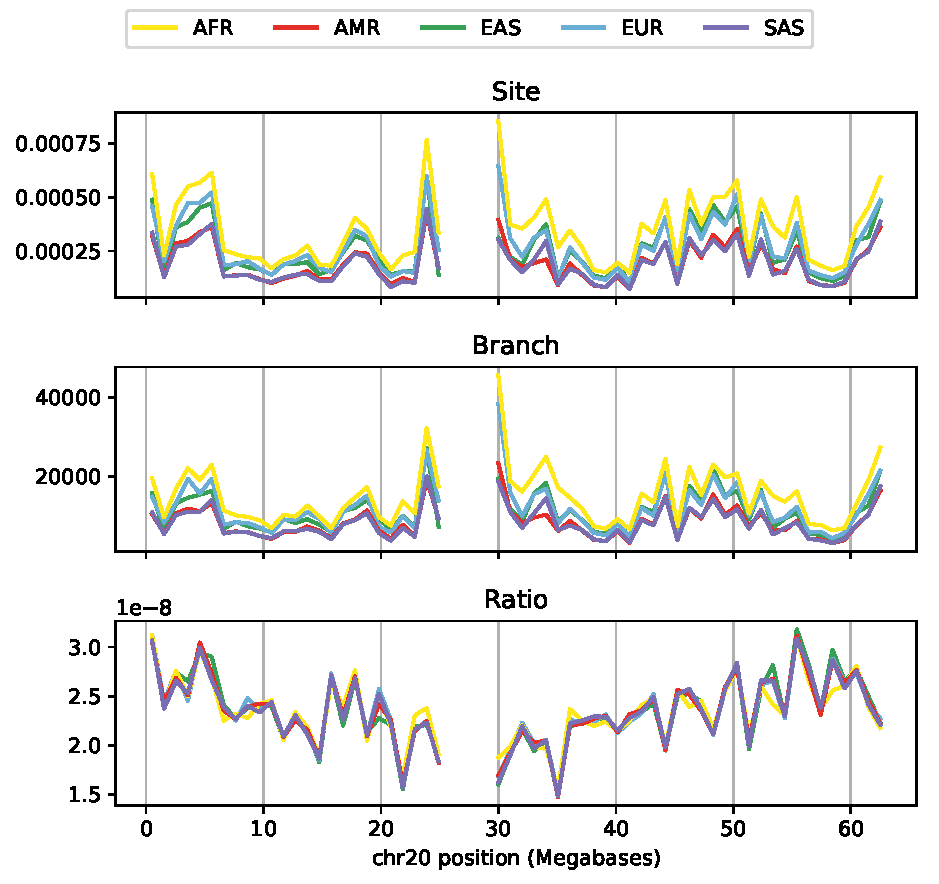
\includegraphics{{figures/1kg/relate_chr20_site_div_branch.1000000.diversity}.pdf}
    \caption{
        \textbf{(top)} Mean sequence diversity
        in 1Mb windows along human chromosome 20 of the 1000 Genomes Project,
        in units of mean number of pairwise differences per nucleotide.
        \textbf{(middle)}
        The dual Branch statistic as calculated from trees inferred by
        Relate~\citep{speidel2019method},
        in units of generations.
        \textbf{(bottom)} The ratio of the Site statistic to the Branch statistic.
        Separate curves are plotted for continental groupings:
        AFR, Africa; AMR, America; EAS, east Asia; EUR, Europe; SAS, south Asia.
        \label{fig:chr20}
    }
\end{figure}

In practice, we do not expect Branch and Site diversity to agree exactly,
because of local differences in mutation rate and intensities of selected mutations.
For instance, regions in which a high proportion of potential mutations are deleterious
are expected to have a lower diversity for two reasons:
first, the deleterious mutations themselves are less likely to be found,
and second, the indirect effect of deleterious mutations on nearby sites reduces typical tree height
and thus diversity at even neutral, linked sites \citep{hudson1994levels,charlesworth1997effects}.
The first effect would cause Site and Branch statistics to differ,
because it effectively reduces the mutation rate in the region
and violates the assumption of independence of mutations given the trees.
However, the second effect does \emph{not} affect the correspondence between Site and Branch statistics,
since it is mediated by tree shape.
It is generally unknown how much mutation rate varies along the genome
\citep[but see][]{supek2015differential}
or how dense targets of selection are~\citep{leffler2012revisiting}.
For this reason, it is very interesting to see how close a correspondence between Site and Branch
statistics it is \emph{possible} to obtain ---
it is tempting to say that the best tree sequence would obtain
as tight a match between Site and Branch statistics as possible,
with remaining variation explained by direct selection and/or mutation rate variation.

% This paragraph is essentially saying the same thing as the previous one,
% so am cutting it. Perhaps we could merge some of the content into the
% the paragtraph above?

% The duality between Site and Branch statistics depends crucially on two assumptions:
% that each new mutation is distinguishable, as in the infinite-sites model,
% and that mutation rates are constant along the genome.
% Neither of these things are true, but are they good approximations?
% Multiple mutations at the same site, causing back mutations,
% are present in real datasets but are generally thought to be uncommon,
% especially if hypervariable sites are excluded.
% The effect of multiple mutations on Site statistics
% can be bounded by a function of the proportion of sites at which these occur.
% Large-scale variation in mutation rate (at, say, the megabase scale)
% might plausibly have a stronger effect on the correspondence,
% because a Branch and Site statistic are equal in expectation up to multiplication by the mutation rate.
% For instance, if we knew that the inferred tree sequences of \autoref{fig:chr20} were correct,
% then dividing the Site statistic by the Branch statistic
% could give us an estimate of relative average mutation rate in windows along the genome.
% Similarly, Branch statistics from well-calibrated tree sequences
% would provide a way to assess variation in population genetic summaries along the genome
% in a way independent of local mutation rate.

A final crucial assumption underlying the duality between Site and Branch
statistics is that mutations can be treated as independent of the trees themselves.
This is clearly not always true --- for instance,
a sweeping beneficial mutation strongly affects the local trees (as in \autoref{fig:sweep_duality}) ---
but seems likely to be approximately true.
\citet{ralph2019empirical} contains more discussion of variation in mutation rate,
but more work needs to be done, particularly on models with large proportions of sites under selection.


%%%%%%%%%%%%%%%%%%
\section*{Algorithm and implementation}

In this section we describe and analyze the algorithm used
to compute Branch statistics. This is a generalization
of the algorithm used to maintain the number of samples from a
given set that derive from each node in a tree
sequence \cite[Algorithm L]{kelleher2016efficient}. The central
problem shared across Site, Branch and Node statistics
is to efficiently maintain the ``state'' $x(u)$ (where $x(u)$ is the
sum of the weights for all samples descending
from, and including, node $u$; see Figure~\ref{fig:adding_weights}).
As we move along the sequence, the trees change when branches are inserted and removed.
By carefully ordering these insertions and removals,
we ensure that this state can be correctly maintained
using only small adjustments for each tree.
Computing the statistics is then a straightforward matter of applying the summary function $f$
to the node states and aggregating the results appropriately for the
particular statistics mode and windowing options.

Formally, we represent a tree sequence using a set of tables~\citep{kelleher2018efficient}.
Each node describes a particular haplotype (i.e., one of the two genomes of a diploid individual),
and details about these haplotypes are stored in a node table, $\Nt$.
The row $\Nt[u]$ contains all information about the node $u$, and rows
are indexed from zero such that $0 \leq u < |\Nt|$.
In particular, the birth time for $u$ is given by $\Nt[u]\prop{time}$.
Information about how nodes relate to each
other along the genome is encoded in an edge table, $\Et$.
For a given row $j$, $\Et[j]\prop{child}$ and $\Et[j]\prop{parent}$
define a parent-child relationship between two nodes in a set of
contiguous trees along the genome. $\Et[j]\prop{left}$ then denotes
the left-most (inclusive) and $\Et[j]\prop{right}$ the right-most
(exclusive) genome coordinates over which this branch exists.
The order in which edges are inserted and removed is determined
by the ``index vectors'' $\indexin$ and $\indexout$~\citep{kelleher2016efficient}.
The ``edge insertion'' vector $\indexin$ gives the ordering of edges
sorted by left endpoint, and among edges with the same left endpoint,
sorted so that edges closer to the root appear later.
The ``edge removal'' vector $\indexout$ is similar, except gives the ordering of edges
by right endpoint and with edges closer to the root appearing sooner.
As we move along the tree sequence, the topology of the current tree is recorded in the
``parent vector'' $\pi$: the parent of each node $u$ is the node $\pi_u$,
with $\pi_u = -1$ if $u$ is a root.
Similarly, we maintain the branch length vector $\beta$ by setting
$\beta_u = \Nt[\pi_u]\prop{time} - \Nt[u]\prop{time}$ and
$\beta_u = 0$ if $u$ is a root. As evaluating the summary function
$f$ is an expensive operation, we also maintain the vector $F$
such that $F_u = f(x_u)$. For notational simplicity here we assume
that weights and summary functions are scalars, but the extension to
vectors is trivial. We also assume that we are computing the statistic
across the full span of the tree sequence; the extension to multiple windows is routine.
See below for a description of the steps in words,
and \autoref{fig:algorithm_example} for an example of the internal state of the algorithm.

\begin{taocpalg}{B}{General Branch statistics}
{Given a list of $n$ sample nodes $S$, corresponding weights $w$ and
summary function $f: \R \rightarrow \R$,
compute the span-normalized statistic $\sigma$
over a tree sequence with sequence length $L$
defined by the node and edge tables $\Nt$ and $\Et$. We assume
that the index vectors $\indexin$ and $\indexout$ have been precomputed.
}

\algstep{B1.}{Initialization.}{
    For $0 \leq u < |\Nt|$ set $\beta_u \leftarrow x_u
    \leftarrow F_u \leftarrow 0$ and $\pi_u \leftarrow -1$.
    Then, for $0 \leq j < n$ set $u \leftarrow S_j$,
    $x_u \leftarrow w_j$ and $F_u \leftarrow f(x_j)$. Finally,
    set $s \leftarrow \sigma \leftarrow j \leftarrow k \leftarrow t_l \leftarrow 0$.
}

\algstep{B2.}{Terminate.}{If $j = |\Et|$ return $\sigma / L$ and terminate.
}

\algstep{B3.}{Edge removal loop.}{If $k = |\Et|$ or $t_l \neq
    \Et[\indexout_k]\prop{right}$ go to \algorithmref{B6}.}

\algstep{B4.}{Remove edge.}{Set
    $u \leftarrow \Et[\indexout_k]\prop{child}$,
    $v \leftarrow \Et[\indexout_k]\prop{parent}$ and $k \leftarrow k + 1$.
    Then set $s \leftarrow s - \beta_u F_u$, $\pi_u \leftarrow -1$
    and $\beta_u \leftarrow 0$.
}

\algstep{B5.}{Propagate loss.}{While $v \neq -1$, set
    $s \leftarrow s - \beta_v F_v$, $x_v \leftarrow x_v - x_u$,
    $F_v \leftarrow f(x_v)$, $s \leftarrow s + \beta_v F_v$
    and $v \leftarrow \pi_v$. Afterwards, go to \algorithmref{B3}.
}

\algstep{B6.}{Edge insertion loop.}{If $j = |\Et|$ or $t_l \neq
    \Et[\indexin_j]\prop{left}$ go to \algorithmref{B9}.}

\algstep{B7.}{Insert edge.}{Set
    $u \leftarrow \Et[\indexin_j]\prop{child}$,
    $v \leftarrow \Et[\indexin_j]\prop{parent}$ and $j \leftarrow j + 1$.
    Then set $\pi_u \leftarrow v$,
    $\beta_u \leftarrow \Nt[v]\prop{time} - \Nt[u]\prop{time}$ and
    $s \leftarrow s + \beta_u F_u$.
}

\algstep{B8.}{Propagate gain.}{While $v \neq -1$, set
    $s \leftarrow s - \beta_v F_v$, $x_v \leftarrow x_v + x_u$,
    $F_v \leftarrow f(x_v)$, $s \leftarrow s + \beta_v F_v$
    and $v \leftarrow \pi_v$. Afterwards, go to \algorithmref{B6}.
}

\algstep{B9.}{Tree loop tail.}{Set $t_r \leftarrow L$.
    If $j < |\Et|$ set $t_r \leftarrow \min(t_r, \Et[\indexin_j]\prop{left})$.
    Then, if $k < |\Et|$ set $t_r \leftarrow \min(t_r, \Et[\indexout_k]\prop{right})$
    Finally, set $\sigma \leftarrow \sigma + (t_r - t_l)s$,  $t_l \leftarrow t_r$
    and go to \algorithmref{B2}.
}

\end{taocpalg}

Algorithm \algorithmref{B} (named ``B'' for ``Branch'')
begins by setting the initial state for $\pi$, $\beta$,
$x$ and $F$ for each node in the tree sequence, and then sets the values
of $x_u$ and $F_u$ for each of the samples $u$ in $S$.
(The initial state is the ``empty forest'', where no nodes are connected to any others.)
Afterwards, we set our ``running sum'' $s$ and output statistic $\sigma$ to zero, along
with the ``tree left'' variable $t_l$. The $j$ and $k$ variables are
used to keep track of our position in the edge insertion and edge
removal indexes, respectively. After completing initialization in
\algorithmref{B1}, we enter the main tree loop in \algorithmref{B2} which is
run once for each tree in the sequence. As we are processing each
tree, we keep track of the edges that need to be processed with
the $t_l$ variable, which stores the left-most genome coordinate
in the current tree. The first thing we do for a new tree is to
remove any edges that were in the previous tree and are not in the
current tree. These must be the edges in which the right coordinate
is equal to $t_l$, and so \algorithmref{B3} loops over these edges using
the edge removal index $\indexout$. Step \algorithmref{B4} then removes
the branch $u \mapsto v$ corresponding to a single edge, by
subtracting its contribution to the running sum $s$, setting the parent of
$u$ to $-1$ and its branch length to $0$. As shown in
Figure~\ref{fig:algorithm_example}B, removing an edge will result
in the subtree rooted at $u$ becoming disconnected from the rest of the
tree. Step \algorithmref{B5} ensures that the state of the rest of the tree
is correctly maintained by propagating the loss of the state $x_u$
up the tree from $v$. Thus, for each node $v$ that was a
direct ancestor of $u$ in the previous tree, we first subtract
its contribution from the running sum $s$ and remove the contribution
of $x_u$ from its state. Since the state of $v$ has changed, we must
recompute the value of our summary cache $F_v$, and then finally
add the new contribution of $v$ to $s$. (For example, note the changes in $x$
and $F$ for nodes 7 and 8 in Figure~\ref{fig:algorithm_example}B.)

Once all of the edges with right coordinate equal to $t_l$ have been removed in
steps \algorithmref{B3--B5}, we then insert edges that start in the current tree
(i.e., with left coordinate $t_l$) in steps \algorithmref{B6--B8}. We update the
state to account for the new branch $u \mapsto v$ by setting the parent of
$u$ to $v$, computing the branch length of $u$ and adding the new contribution
of $u$ to $s$ in \algorithmref{B7}. Then, as adding a new edge can connect the
subtree rooted at $u$ to the larger tree at $v$, we propagate the gain of $x_u$
up the tree in step \algorithmref{B8} (note the symmetry with step \algorithmref{B5}).
Finally, once we have removed and inserted all of the relevant edges, we are
ready to add the contribution of the current tree to the overall statistic,
$\sigma$ and move on to the next tree in step \algorithmref{B9}. To do this, we first
compute the right-hand coordinate of the tree $t_r$ (a process slightly
complicated by the possible presence of ``gaps'' in the tree sequence, spanned
by no edges). Then, we add the running sum $s$ weighted by the span of the
current tree $t_r - t_l$ to $\sigma$, and return to \algorithmref{B2} to process the
next tree. If we have reached the end of the sequence, we then divide $\sigma$
by the sequence length to normalize and exit.

To analyze Algorithm~\algorithmref{B} we will assume that the tree sequence has
been simulated under the standard coalescent with a sample of size
$n$ and population scaled recombination rate $\rho = 4 N_e r$,
where $r$ is the mean number of recombinations per chromosome per unit of time.
Under these conditions, there are $O(n + \rho \log n)$ edges in the tree sequence
\citep{kelleher2016efficient}.  Clearly, each edge is examined
exactly once in steps \algorithmref{B6} and \algorithmref{B7} in order to create
the trees, and at most once in steps \algorithmref{B3} and \algorithmref{B4} (we do
not remove the edges for the final tree). Additionally, each edge that
we insert or remove after the initial building of the tree
may incur the cost of traversing up the tree as
far as the root in steps \algorithmref{B5} and \algorithmref{B8}.
As coalescent genealogies are asymptotically
balanced \citep{li2013coalescent}, the expected number of nodes
on the path to root is $\log_2 n$.
Therefore, the overall running time
of Algorithms~\algorithmref{B} is of order $n + \rho \log(n) \log_2(n)$, which is
\begin{equation}\label{eqn:alg_complexity}
    O\left(n + \rho \log(n)^2 \right).
\end{equation}
Computing a Site statistic will have the same complexity,
as the same internal state is maintained,
and the number of segregating sites is proportional to the number of edges
(with constant equal to the ratio of mutation to recombination rate).
The asymptotic analysis here assumes that we traverse upwards to root
for each edge, but this is not the case. Edges are removed in
oldest-first order, guaranteeing that the deepest node any subtree being
modified is processed first. Therefore, this subtree will be disconnected from the
main tree, ensuring that we traverse upwards all the way to root only once.
Similarly, edges are inserted in youngest-first order, ensuring that subtrees are only
reconnected to the main tree when they are fully built.

\begin{figure}
\footnotesize
    % Run the script illustrate_algorithm.py to generate these pdfs and
    % the latex tables below.
    \begin{center}
    \begin{tabular}{ccc}
    \includegraphics[width=4cm]{figures/tree_0_init.pdf} & &
    \includegraphics[width=4cm]{figures/tree_0_out_0.pdf}
    \\
    $s = 3.1$ & & $s = 2.9$\\

    \begin{tabular}{c|cccc}
    & $\pi$ & $\beta$ & $x$ & $F$\\
    \hline
    0 & 8 & 4.0 & 1.0 & 0.2\\
    1 & 5 & 1.0 & 1.0 & 0.2\\
    2 & 5 & 1.0 & 1.0 & 0.2\\
    3 & 6 & 2.0 & 1.0 & 0.2\\
    4 & 6 & 2.0 & 1.0 & 0.2\\
    5 & 7 & 2.0 & 2.0 & 0.3\\
    6 & 7 & 1.0 & 2.0 & 0.3\\
    7 & 8 & 1.0 & 4.0 & 0.2\\
    8 & -1 & 0.0 & 5.0 & 0.0\\
    \end{tabular}
    & &
    \begin{tabular}{c|cccc}
    & $\pi$ & $\beta$ & $x$ & $F$\\
    \hline
    0 & 8 & 4.0 & 1.0 & 0.2\\
    1 & 5 & 1.0 & 1.0 & 0.2\\
    2 & 5 & 1.0 & 1.0 & 0.2\\
    3 & 6 & 2.0 & 1.0 & 0.2\\
    4 & 6 & 2.0 & 1.0 & 0.2\\
    5 & 7 & 2.0 & 2.0 & 0.3\\
    6 & -1 & 0.0 & 2.0 & 0.3\\
    7 & 8 & 1.0 & 2.0 & 0.3\\
    8 & -1 & 0.0 & 3.0 & 0.3\\
    \end{tabular}
    \\
    (A) && (B)
    \end{tabular}
    \end{center}

    \caption{
    Illustration of the internal state for algorithm B for $\iw = \bone_S$ and
    $f(x) = x(5 - x) / 20$ as in Example~\ref{ex:site_diversity}. (A)
    Immediately before we remove the edge joining 6 to 7 and (B) immediately after.
    See the text for descriptions of the arrays encoding the state. Also shown
    is the value of the running sum, $s = \sum_u \beta_u F_u$.
    \label{fig:algorithm_example}}
\end{figure}

The tree sequence describes trees that change as one moves along the genome,
and so is a special case of a \emph{dynamic graph},
also called a \emph{graph timeline} \citep{lacki2013reachability}.
Much of the work on dynamic graphs is focused on connectivity,
e.g., maintaining a minimum spanning tree \citep{eppstein1994offline, eppstein1997sparsification, holm2001polylogarithmic},
but development of parallel algorithms for more general operations on large dynamic graphs
is an active area of research \citep[e.g.,][]{srinivasan2018sharedmemory}.
An interesting direction for future work is to develop
parallel versions of tree sequence algorithms such as Algorithm B.

%%%%%%%%%%%%%%%%%%%%%
\subsection*{Efficiency}

We used coalescent simulations to compare the performance of calculating Tajima's \citeyearpar{Tajima1989-de} $D$
statistic from tree sequences to calculating it from integer matrices containing genotypes at all variable positions.
\autoref{fig:stats_performance} shows that the tree sequence methods implemented in \texttt{tskit} processes variant data
substantially faster than matrix-based approaches once the sample size is above $n \approx 500$ haploids ---
three times faster for one thousand haplotypes,
growing to nearly three orders of magnitude faster for one million haplotypes.
The expected number of mutations for each replicate is $10^4 \times \sum_{i=1}^{n-1}\frac{1}{i}$, and thus ranges from
$\approx 32,000$ to $\approx 138,000$ \citep{Watterson1975-ej}.
\autoref{fig:stats_performance} only considers the time required to calculate the statistic
once the data is present in each library's native format.
For the largest samples size of $n=10^6$,
the matrix is approximately 200 gigabytes, and thus not practical on many systems.
The largest tree sequence simulated required less than one gigabyte of memory.

To determine how well our theoretical model of time complexity predicts the
running time in \tskit{}'s implementation of the Site statistics algorithm,
we fit a model based on Equation~\eqref{eqn:alg_complexity}.
\autoref{fig:stats_performance} shows that theoretical predictions match
the observed running time very well. As the overall complexity is
$O(n + \rho \log(n)^2)$, for sufficiently large $n$ the initial term
(representing the cost of building the first tree) will come to dominate.
In our simulations, we can see this happening at around $n = 10^5$, where there
is a noticeable uptick in the time required per variant. For
longer genomes (i.e., larger values of $\rho$), this cost is amortized over more trees
and is less apparent.

\begin{figure}
    \centering
    \includegraphics[width=9cm]{tskit_stat_benchmarks/benchmarks_without_copy_longer_genome.pdf}
    \caption{Comparison of time required to compute Site statistics
        between matrix and tree based methods. For each sample size, a single replicate
        was obtained using \texttt{msprime} with scaled neutral mutation rate $\theta = 4 N_e L \mu$ and
        scaled recombination rate $\rho = 4N_er$ both equal to $10^4$ and $N_e = 10^4$,
        where $L\mu$ and $\rho$ are the total mutation and recombination rate across the simulated region
        per generation, respectively.
        For each replicate, Tajima's $D$
        \citep{Tajima1989-de} statistic was calculated using \tskit, \texttt{libsequence}
        \citep{Thornton2003-wj}, and \texttt{scikit-allel} \citep{miles2017scikit}.
        The solid green line shows the result of fitting the timing data to a model based on the expected complexity of the algorithm used by \texttt{tskit}
        (\autoref{eqn:alg_complexity}).
        \label{fig:stats_performance}
    }
\end{figure}

It should be noted here that this example based on simulated data
represents a best-case scenario in terms of the performance advantages
of \tskit{} over the matrix-based methods. For real data, inferred
tree sequences currently contain substantially more edges than we
would expect based on simple neutral theory~\citep{kelleher2019inferring},
and therefore computing statistics will not be as efficient as
for an equivalent simulation. Tree sequence inference
methods are in their infancy, however, and it is likely that
as they improve the number of edges required to encode data will
be reduced. For data simulated natively in tree sequence format
via packages such as \texttt{msprime}~\citep{kelleher2016efficient},
\texttt{SLiM}~\citep{haller2018tree,haller2019slim} and
\texttt{fwdpy11}~\citep{thornton2014c++}, however, the advice is straightforward.
Computing statistics using the algorithms in \tskit{}
will always be more efficient than decoding the genotype
matrix, importing it into another package and computing from the matrix.



%%%%%%%%%%%%%%%%%%%%%%%
\section*{Discussion}

% overview: general definition that is mostly functions of jAFS but includes others
In this paper we have described a general framework for summarizing genetic variation
and the underlying genealogies
that encompasses many standard population genetic statistics.
Many of these statistics are functions of the joint allele frequency spectrum,
but the framework is more general and can be used,
for example, to quantify associations between genotypes and phenotypes.
This generality greatly reduces the software development effort in
implementing statistics efficiently,
and it also allows users to easily explore new classes of statistics.
The range of statistics available to describe variation in a single exchangeable sample
(e.g., an isolated population) are well-understood
\citep{achaz2009frequency,ferretti2017decomposing},
but there are much larger and less well-explored classes of statistics
describing genetic variation between many populations
or across geographical space.
The statistics defined here are all additive along the genome:
if we have computed a statistic in equal-size windows along a chromosome,
then the value of the statistic for the entire chromosome is equal to
the average of the values in those windows.
Some commonly-used statistics (e.g., $F_{ST}$ or Tajima's $D$)
are not additive, but are ratios of additive statistics, so can be easily computed in this way.
% We have also defined site statistics to be additive across \emph{alleles},
% to allow the definitions to apply to sites with more than two alleles.
% This decision has some nice properties, but is not the only reasonable choice.
% Multilocus statistics that measure linkage disequilibrium or haplotype lengths
% do not fall in this category.
Extensions to statistics involving the pairwise joint distribution of genotypes across
sites~\citep{hudson2001twolocus} such as linkage disequilibrium are planned for future work.
Haplotype-based statistics may require different classes of algorithms.

% jk: Cut this: too technical for the discussion
% We also require that Site statistics be computable from the genotype matrix
% (i.e., without knowledge of the trees),
% and, if the statistic is polarized, knowledge of the ancestral allele.
% We often would also like our statistics to be unaffected by the addition of monomorphic sites,
% which are usually omitted from genetic variation data.
% To ensure this we have required that the summary function returns zero when give both zero weight
% and the total weight: $f(0) = f(\tiw) = 0$.
% This also makes Branch and Node statistics unchanged by portions of the tree that do not lie on a path
% between any of the samples that have nonzero weight,
% so that in particular,
% \emph{simplification} of the tree sequence will not change the value of the statistic.
% However, in practice this requirement can be relaxed.


% speed/efficiency: big data sets; large simulations
The most obvious application of these methods on current practice
is to improve efficiency of existing pipelines,
as tree sequences allow storage and processing of large genomic data sets
with orders of magnitude less space and time than standard matrix-based methods.
All statistics described here (and more) are implemented
in the rigorously tested \tskit{} library,
which provides a suite of tools for working with tree sequences in Python and C.
Large-scale simulations are useful in many contexts
\citep[e.g.,][]{martin2017human,browning2018one,galloway2019stickleback}
and the ability to quickly compute a wide range of statistics from
these (previously prohibitively large) datasets opens up new possibilities.
At smaller scales the statistics are still highly efficient, and avoiding
the cost of exporting simulated data to a genotype matrix will in practice greatly
speed up inference based on summaries computed from simulated
data~\citep{beaumont2002approximate,csillery2010approximate,schrider2018supervised}.
Efficient simulations coupled with the framework developed here allow us to
explore the full distribution of summaries along the genome, which has
important applications in (e.g.) speciation genomics~\citep{lohse2017come}.
The ability to efficiently compute statistics from real data is, of course, also welcome.

The correspondence between genome sequence and properties of the
underlying genealogies we have used here is well-known,
and is the basis for several inference methods~\citep{becquet2007new,beeravolu2018able}.
The general framework
that we have defined, however, codifies this relationship in a
mathematically elegant and computationally efficient way, and may lead to
new perspectives on well-studied problems.
One way to use the duality between Site and Branch statistics is to answer:
what aspect of tree shape is a particular population genetics statistic summarizing?
This can help when interpreting results, especially if reality may not fit an idealized model
of separate populations.
However, methods to infer tree sequences from real data
make it now possible to work in the other direction:
instead of calculating (Site) statistics from the genotype matrix,
we can calculate precisely analogous (Branch) statistics from the trees themselves,
thus hopefully bypassing the extra layer of noise induced by mutation.
How well this works will depend on the ability of inference methods
to estimate the true tree sequence.
This might plausibly produce less noisy estimates because tree sequence inference
should use the signal from nearby patterns of variation
to interpret relationships at a given site,
thus transforming the simple binary split induced by a SNP
into a much richer source of information.
Furthermore,
if tree sequence inference can be made insensitive to local variation in mutation rate,
calculation of Branch statistics would provide a summary method
that is not affected by this potentially important confounding factor.
Similarly, if tree sequences inferred from
genotype array data~\citep{kelleher2019inferring} are unbiased,
then Branch statistics could provide a way
to estimate genome-wide quantities without ascertainment bias.
This procedure would be similar to imputation, and would likely face similar challenges.

% duality: site stats ~ branch stat, but conversely branch more accurate version of site
%  maybe analogous to imputation
% Not sure about this: tangent? Perhaps combine this point with some others
% in a compressed form?
% Many genomic datasets only contain genotype information at a subset of sites
% that do not represent an unbiased look at genome-wide variation,
% introducing an ascertainment bias that is difficult to account for in for many applications.
% If, however, unbiased tree sequences can be inferred using these data,
% then Branch statistics could provide unbiased estimates of genome-wide quantities.
% This is in principle possible, as \citet{kelleher2019inferring} inferred tree sequences
% with UK BioBank data, produced using genotyping arrays \citep{bycroft2018genome}.
% This procedure would be similar to imputation, and would likely face similar challenges.

% visualization and time decomposition adding a new dimension
Genomic data are naturally distributed on two axes: along the genome, and across geography.
The tree sequence extends this to a third axis: time.
A great many methods in population genetics aim to describe aspects of history,
and accurate (or at least unbiased) tree sequence inference
may shift the focus of these problems from inference to descriptive analysis.
The methods developed here distribute the contribution to various statistics across each tree,
and so could also be used to summarize contributions to various statistics across time.
This could provide, for instance, the time distribution of mutations or branches
contributing positively or negatively to $f_4$ statistics of introgression,
enabling historical interpretations of these signals.
% This additional mode of reporting statistics is an important subject for future work.
% moving past a few summaries in discrete groups to a genome/time/space view of relatedness
The computational toolbox of population genetics
is still mostly composed of statistics originally designed for analysis of a handful of loci
in a small number of discrete, mostly separated populations.
Both our data and our understanding of the world have moved beyond this.
We hope that the tools developed here will help make it possible
to visualize and analyze genetic variation and genealogical relatedness
along the genome, across space, and through time.

%%%%%%%%%%%%%%%%%%
% \subsection*{Duality in practice?}
% Moved this to the 1000G section where we're already discussing it.

%%%%%%%%%%%%%%%%%%
% \subsection*{General properties}

% Merged in with disco content above.

%%%%%%%%%%%%%%%%%%
% Moved this content into the "Algorithms" section
% \subsection*{Dynamic graph algorithms}


%%%%%%%%%%%%%%%%%%%%%%%
\subsection*{Acknowledgments}
Thanks to Georgia Tsambos, Graham Coop, Andrew Kern, Nick Patterson, Kelley Harris,
Aaron Ragsdale, Konrad Lohse, and Wilder Wohns for useful suggestions
and to Leo Speidel for providing the inferred 1000 Genomes trees.
This work was supported by NSF grant \#1262645 (DBI) to PLR
and by NIH grant R01-GM115564 to KRT. JK was supported by
the Robertson Foundation and Wellcome Trust grant 100956/Z/13/Z
to Gil McVean.

\paragraph{Author contributions}
Designed the study: PR, JK. Wrote the code: PR, JK. Carried out the experiments: PR, KT, JK. Wrote the paper: PR, KT, JK.

\bibliography{references}

\clearpage
\appendix
\setcounter{table}{0}
\renewcommand{\thetable}{S\arabic{table}}
\setcounter{figure}{0}
\renewcommand{\thefigure}{S\arabic{figure}}




%%%%%%%%%%%
\appendix

\section{Linear regression}
\label{apx:regression}

Let $h$ be a trait, $Z$ be a matrix of covariates, and $g$ be a vector denoting inheritance
(so, with $n$ samples, $h$ and $g$ are both $n$-vectors and $Z$ is an $n \times k$ matrix).
We would like to find the coefficient of $g$ in the linear regression of $h$ against $g$ and $Z$,
without doing full multivariate regression for every new $g$,
using the fact that $Z$ is always the same.
Suppose that $Z^T Z = I$ and that the vector of all ones is in the span of the columns of $Z$,
although in the implementation we post-process $Z$ to make this the case.
Then, let $a$ be the number and $b$ be the $k$-vector satisfying
\begin{align*}
    a, b = \text{argmin}\left\{ \sum_i \left( w_i - a g_i - \sum_j Z_{ij} b_j \right)^2 \right\}
\end{align*}
Our goal is to compute $a$.
Writing this in block matrix notation, $a$ and $b$ minimize
\begin{align*}
    \left\|
        \left[ \begin{array}{@{}c@{}} h \end{array}\right]
            -
        \left[ \begin{array}{@{}c|c@{}} g & Z \end{array} \right]
            \left[ \begin{array}{@{}c@{}} a \\ \hline b \end{array} \right]
    \right\|^2 .
\end{align*}


Letting $B = [g | Z]$, the solution to this is
\begin{align*}
    \left[\begin{array}{@{}c@{}}a\\\hline b\end{array}\right]
        = (B^T B)^{-1} B^T h ,
\end{align*}
as long as $B^T B$ is invertible (which we assume to be the case).
Let $m = g^T g$ be the number of alleles in the sample coded 1,
let $u = g^T Z$ be the vector giving sums of the covariates of all samples carrying the allele,
and
\begin{align*}
    \alpha
    &=
        (g^T g - g^T Z (Z^T Z)^{-1} Z^T g) \\
    &=
        m - \sum_j u_j^2 .
\end{align*}
$\alpha$ is the norm of the component of $g$ not in the subspace spanned by the columns of $Z$,
so if $\alpha = 0$ then we want to return $a=0$.

Otherwise, by the inversion formula for a block two-by-two matrix,
since we have assumed that that $Z^T Z = I$,
\begin{align*}
    (B^T B)^{-1}
    &=
    \left[
        \begin{array}{@{}cc@{}}
            m & u \\
            u^T & I
        \end{array}
    \right]^{-1} \\
    &=
    \left[
        \begin{array}{@{}cc@{}}
            1/\alpha
            &
            - u / \alpha
            \\
            - u^T / \alpha
            &
            m \left(m I - u u^T \right)^{-1}
        \end{array}
    \right] .
\end{align*}
Now, the regression coefficient we seek is,
with $h_g = g^T h$,
\begin{align*}
    a
    &=
    \frac{1}{\alpha} \left(
        h_g - u Z^T h
    \right) .
\end{align*}

To compute this in the framework above,
first add a column of 1s to the covariates $Z$,
then decorrelate the resulting matrix, so that now $Z^T Z = I$.
Then, put this normalized version of $Z$
into the first $k$ columns of the weight matrix (so that $w_j(u) = Z_{uj}$),
set the $(k+1)^\text{st}$ column to the trait (so that $w_{k+1}(u) = w_u$),
and the final column to all $1$s (so $w_{k+2}(u) = 1$).
Also let $Z^T h = v$ be precomputed.
Then the sum of the traits of samples with the focal genotype is $h_g = x_{k+1}$,
and the allele count is $m = x_{k+2}$,
so that
\begin{align*}
    a
    &=
    \frac{
        h_g - \sum_{j=1}^k x_j v_j
    }{
        m - \sum_{j=1}^k x_j^2 } .
\end{align*}

In practice we square this and divide by two,
so that for biallelic loci the two alleles contribute an equal amount.
For loci with more than two alleles,
it would be more satisfying to return the proportion of variance in the trait
that is explained by \emph{all} of the alleles;
however, this would be more involved
(it would entail inversion of a $3 \times 3$ matrix for each locus).

% # NUMERICAL CHECK
% n <- 20
% k <- 5
% h <- rnorm(n)
% g <- rbinom(n, size=1, prob=0.5)
% oZ <- cbind(matrix(rnorm(n*k), nrow=n), rep(1,n))
% colnames(oZ) <- c(paste0("oZ", 1:k), "1")
% Z <- oZ %*% solve(chol(crossprod(oZ)))
% colnames(Z) <- paste0("Z", 1:(k+1))
% lm_a <- coef(lm(h ~ g + oZ))[2]
% hg <- sum(g*h)
% hZ <- crossprod(Z, h)
% u <- crossprod(Z, g)
% p <- sum(g)
% alpha <- (p - sum(u^2))
% a <- (1/alpha) * (hg - crossprod(u, hZ))
%
% # check formula for regression coefs
% # and that coefficient of g doesn't change on linear transform of Z
% B <- cbind(g, Z)
% H <- cbind(solve(crossprod(B), crossprod(B, h)),
%            coef(lm(h ~ g + Z + 0)),
%            coef(lm(h ~ g + oZ + 0)))
% stopifnot(all(abs(diff(H[1,])) < 2e-15))
% # check for alpha, an other bits
% stopifnot(all(abs(crossprod(B, h) - c(hg, hZ)) < 2e-15))
% stopifnot(all(abs(- (1/alpha) * u - solve(crossprod(B))[1,-1]) < 2e-15))
% stopifnot(abs(solve(crossprod(B))[1,1] - (1/alpha)) < 2e-15)
% stopifnot(all(abs(p*solve(p*diag(k+1) - tcrossprod(u)) - solve(crossprod(B))[-1,-1]) < 2e-15))
% # and the final answer
% stopifnot(abs(a - lm_a) < 2e-15)

\clearpage
\newpage
\section*{Supplementary figures}

\begin{figure}[!h]
    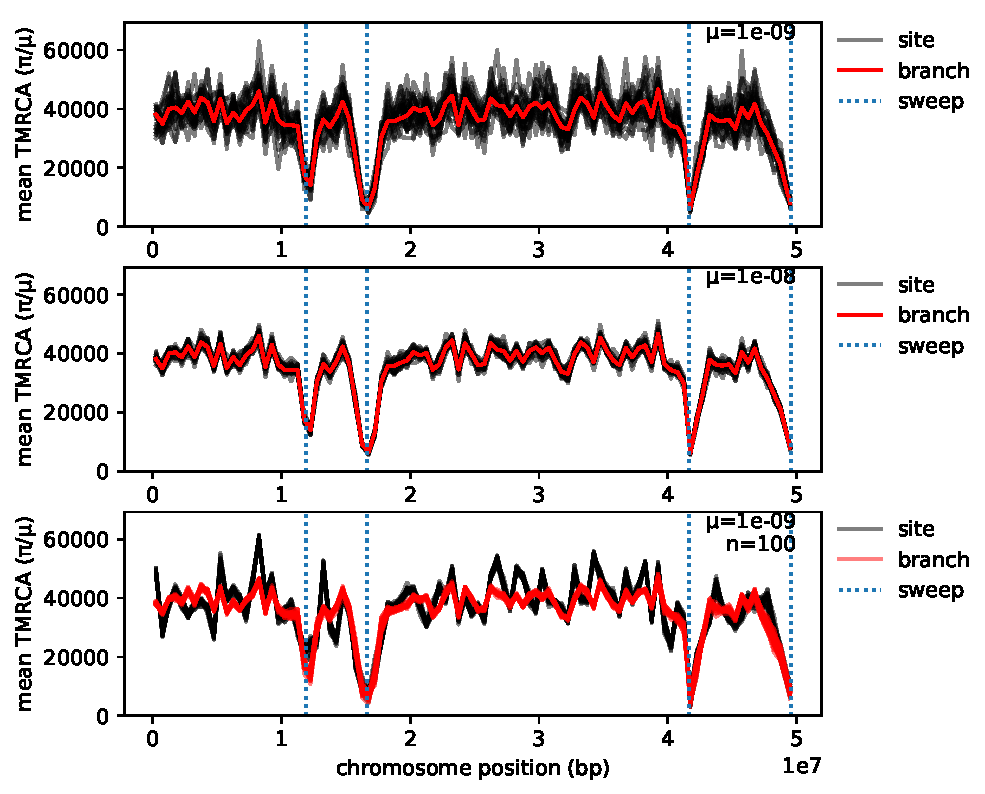
\includegraphics[width=\textwidth]{{figures/swept.10000.765.1e-09.diversity}.pdf}
    \caption{
        As in \autoref{fig:sweep_duality}, but in a population of size 10,000.
        \label{sfig:sweep_duality_10K}
    }
\end{figure}

\begin{figure}[!h]
    \includegraphics[width=\textwidth]{{figures/intro/introgressed.1000.23.1000000.1e-09.f4}.pdf}
    \caption{
        Values of the $f_4$ statistic in megabase windows along the genome
        from the simulations of introgression described in the text.
        Statistics are shown in units of generations:
        Branch statistics are computed in units of time, which is in generations for these simulations;
        and Site statistics are reported in units of mutations per unit of sequence length,
        which we divide by mutation rate per unit of sequence length and per generation
        to obtain units of generations.
        \label{fig:introf4}
    }
\end{figure}

\begin{figure}[!h]
    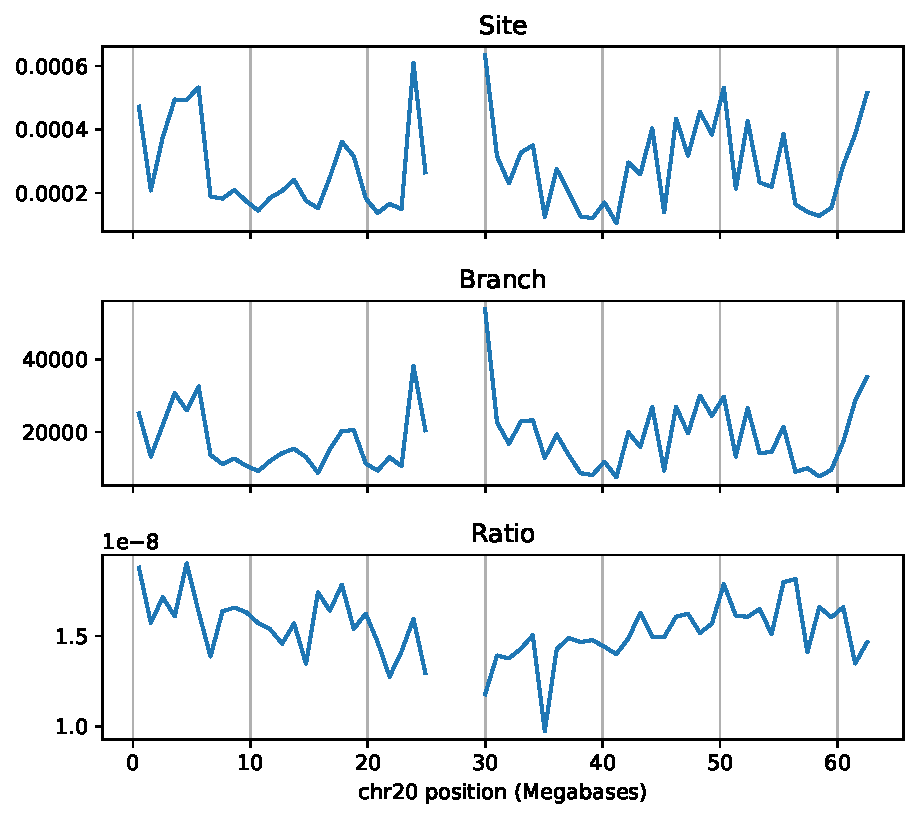
\includegraphics[width=\textwidth]{{figures/1kg/relate_chr20_GBR.branch.1000000.site.ratio}.pdf}
    \caption{
        \textbf{(top)} Mean sequence diversity
        in 1Mb windows along human chromosome 20 of the GBR (Great Britain)
        sample of the 1000 Genomes Project,
        in units of mean number of pairwise differences per nucleotide.
        \textbf{(middle)}
        The dual Branch statistic as calculated from trees inferred by
        Relate~\citep{speidel2019method},
        in units of generations.
        \textbf{(bottom)} The ratio of the Site statistic to the Branch statistic.
        This figure differs from \autoref{fig:chr20} in that the trees were inferred
        using only GBR samples, and Relate was allowed to co-estimate population size and branch lengths,
        with mutation rate fixed at $1.45 \times 10^{-8}$ mutations per generation;
        the trees shown in \autoref{fig:chr20} were inferred with a fixed effective population size
        of $N_e = 15,000$.
        \label{fig:chr20_GBR}
    }
\end{figure}



\end{document}

\paragraph{Diploid statistics}
The statistics we develop here are in essence \emph{haploid} statistics.
These tools can be used to compute a statistic about polyploid individuals,
but they do not scale to large numbers of individuals.
For instance, to compute the heterozygosity of a set of samples
-- this is $(1/N) \sum_{i=1}^N 2 p_i (1-p_i)$, where $p_i$ is the derived allele frequency
in the $i^\text{th}$ individual --
one would need to have an entry in the weight vector for \emph{each individual}.
The genotype of a diploid at a site with a single mutation that occurred on the branch ancestral to node $n$
is determined by where that node falls relative to the diploid's two haplotypes in the tree:
if $n$ is on the path from either haplotype to their MRCA, the individual is heterozygous;
if $n$ is on the path from the MRCA to the root, the individual is homozygous derived;
and the individual is homozygous ancestral otherwise.
This suggests the following generalization of our current scheme for diploids:
for a list $(I_1, \ldots, I_N)$ of pairs of nodes,
and two vectors $w^{(1)}$ and $w^{(2)}$ of weights of length $N$,
add weight $w^{(1)}_i$ to each node on the path between the two nodes of $I_i$,
and weight $w^{(2)}_i$ to each node on the path from the MRCA of $I_i$ to the root.
With $k$ such weighting schemes, we would then need the summary function $F$
to take $k \times 2$ values as input.
Efficiently updating these ``diploid'' weights on the nodes should be possible,
but is not a straightforward extension of our current method.
